\vspace{0.015\textheight}
The physical process under investigation in this thesis is the production of a photon + jet(s) + \met from some mechanism other than the Standard Model. The event signature (i.e.~the set of ``objects'' that we search for in each collision event) consists of a photon, one or more jets, and \met. A \textit{background} is a process that is different from the process under investigation but has the same event signature.

There are different types of backgrounds. In this analysis, every effort is made to identify events with a prompt photon from the hard scattering process. This is done by identifying what appear to be \newterm{isolated photons} in the detector. However, not all objects that appear to be isolated photons in the detector are actually prompt photons from the hard scattering process. Particles can be misidentified due to imperfections in the detector and inefficiencies in the identification requirements. For example, the failure to reconstruct the associated track of an electron may cause it to be identified as a photon. \newterm{Fake photons} are a significant source of contamination in the data sample. In another type of background, the identified particle might in fact be a photon, but not a prompt photon from the hard scattering process. An example is that of a quark or gluon that originates from the hard scattering process and hadronizes into particles including a light meson that eventually decays into one or more photons. Yet another scenario is the production of an actual prompt photon in a hard scattering process that is different from the process under investigation. In this case, the background process is fundamentally indistinguishable.% and thereby \newterm{irreducible}.

All of these backgrounds need to be studied and their effects understood in detail. These backgrounds are estimated and modeled using control samples.

\section{Background Modeling}

Backgrounds for the $\gamma$ + jets signature come from two main sources: SM processes and non-collision processes. The SM processes include prompt $\gamma$ production, prompt diphoton production, electroweak production of charged leptons that fake a prompt photon, and QCD production of hadronic jets that fake a prompt photon. The non-collision processes include energetic particles from both cosmic rays and the beam halo that mimic the signal of a prompt photon from a $p\bar{p}$ collision. The \pythiaText Monte Carlo generator (Tune~A) \cite{pap:PythiaManual} is used to model SM prompt $\gamma$ production, prompt diphoton production, and the electroweak charged lepton backgrounds. All other backgrounds are modeled using data. For each of these SM backgrounds and the combined non-collision background, a background template is derived for each of the kinematic distributions under investigation. The sum of these background templates is then compared to data.

Two different methods of determining the backgrounds, referred to as \newterm{Method A} and \newterm{Method B}, have been developed to better understand the measurements. In the first method (Method A), \pythiaText is used exclusively to predict the kinematic properties of jets in SM $\gamma$ + jets events. In the second method (Method B), a novel weighting technique that uses a combination of data and \pythiaText Monte Carlo is used to model higher-order QCD effects in kinematic distributions involving jets. The two methods differ in their treatment of the SM $\gamma$ background and the QCD multijet background, as described below.

%%%%%%%%%%%%%%%%%%%%%%%%%%%%%%%%%%%%%%%%%%%%%%%%%%%%%%%%%%%%%%%%%%%%%
%          METHOD A
%%%%%%%%%%%%%%%%%%%%%%%%%%%%%%%%%%%%%%%%%%%%%%%%%%%%%%%%%%%%%%%%%%%%%

\section{Method A}\label{sec:MethodA}
In Method A, SM $\gamma$ and QCD multijet background templates are scaled so that the total number of SM $\gamma$ events ($N^\mathrm{SM\gamma}$) and the total number of QCD multijet events ($N^\mathrm{QCD}$) satisfy
\begin{equation}
N^\mathrm{QCD} = f \cdot (N^\mathrm{SM\gamma}+N^\mathrm{QCD}),\label{eqa:SMQCDscaling}
\end{equation}
where $f$ is the fake photon fraction, which is determined to be
\begin{equation}
f~=~\mbox{0.319 $\pm$ 0.001(stat) $\pm$ 0.0068(syst)}
\label{eqa:FakeFraction}
\end{equation}
from a study of inclusive photon data with photon \mbox{\et$>$ 30~\etUnits} \cite{pap:PhotonIDAndCESCPR}. A mathematical overview of the calculation of the fake photon fraction is described in Appendix~\ref{app:CESCPRMtd}. In addition, the overall normalization of the SM $\gamma$ and QCD templates is adjusted so that the total number of background events from all sources equals the number of observed events in the data:
\begin{equation}
 N^\mathrm{Data} = N^\mathrm{SM\gamma}+N^\mathrm{QCD}+\underbrace{N^\mathrm{Di-\gamma}}_{fixed}+\underbrace{N^\mathrm{EWK}}_{fixed}+\underbrace{N^\mathrm{Non-collision}}_{fixed}\, 
\label{eqa:MtdANorm}
\end{equation}
where $N^\mathrm{Data}$ is the total number of data events, $N^\mathrm{SM\gamma}$ is the expected number of SM $\gamma$ events, $N^\mathrm{QCD}$ is the expected number of QCD multijet events, $N^\mathrm{Di-\gamma}$ is the expected number of diphoton events, $N^\mathrm{EWK}$ is the expected number of electroweak events, and $N^\mathrm{Non-collision}$ is the expected number of non-collision events. The exact calculations of these events will be described in the following sections.

When used together, Eqs.~\ref{eqa:SMQCDscaling} and \ref{eqa:MtdANorm} uniquely determine $N^\mathrm{SM\gamma}$ and $N^\mathrm{QCD}$. Note that since the total number of events in the templates is constrained to match the total number of events in the data, the measured kinematic distributions are not sensitive to anomalies in the overall number of \phojets events, but they are sensitive to anomalies in the shapes of the distributions and excesses in the tails.


%%%%%%%%%%%%%%%%%%%%%%%%%%%%%% SM Photon background
\subsection{SM Prompt Photon + Jets Background}\label{sec:SMpromptPhotonJets}

\begin{figure}[p]
\begin{center}
\subfigure[Annihilation]{
\label{fig:SM_pj_annihilation_copy}
\begin{tabular}{cc}
\raisebox{0\height}{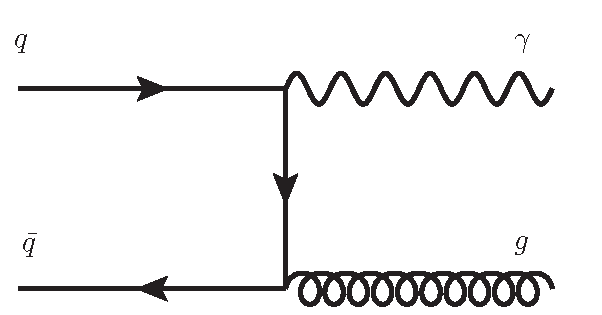
\includegraphics[scale=0.5]{images/Feyn_gjet_annihilation.pdf}} &
\raisebox{0\height}{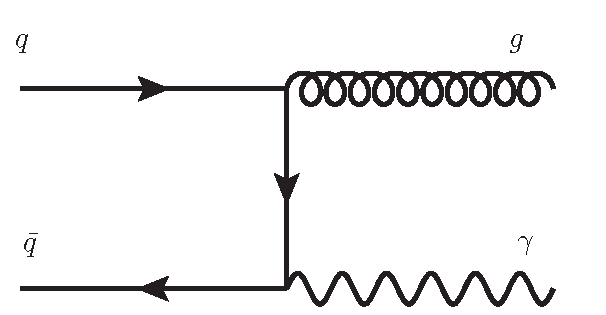
\includegraphics[scale=0.5]{images/gjets_qq2gpho_annihilation3.pdf}}\\
\multicolumn{2}{c}{\raisebox{0\height}{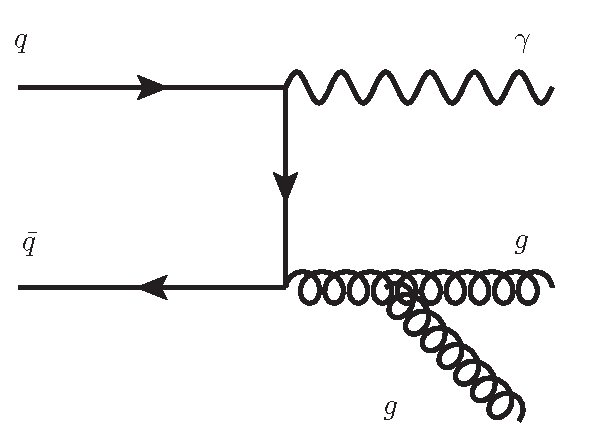
\includegraphics[scale=0.5]{images/Feyn_gjets_annihilation.pdf}}}
\end{tabular}
}
\subfigure[Compton Scattering]{
\label{fig:SM_pj_compton_copy}
\begin{tabular}{cc}
\raisebox{0.1\height}{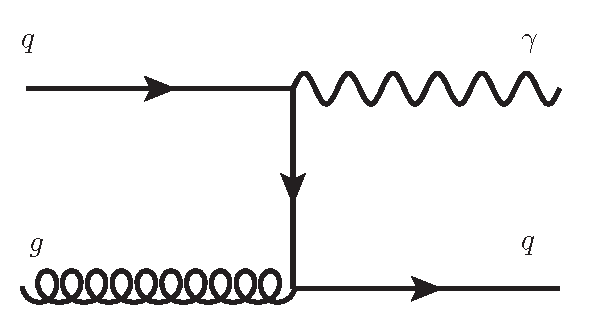
\includegraphics[scale=0.5]{images/Feyn_gjet_compton.pdf}} &
\raisebox{0.0\height}{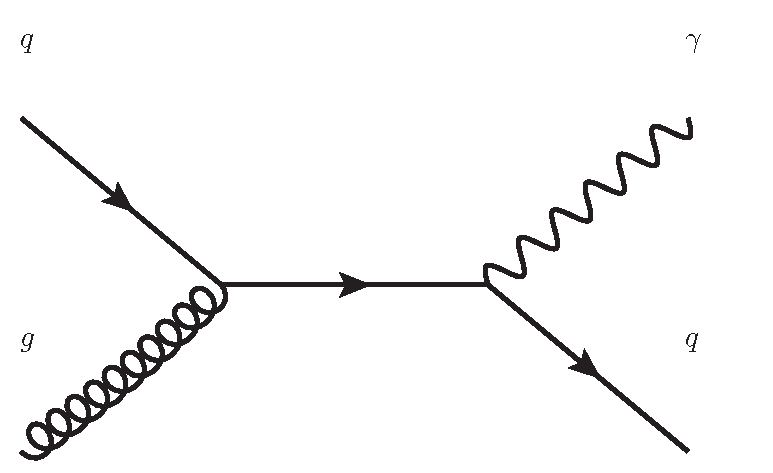
\includegraphics[scale=0.4]{images/gjets_qg2phoq_compton2.pdf}}\\
\raisebox{0.0\height}{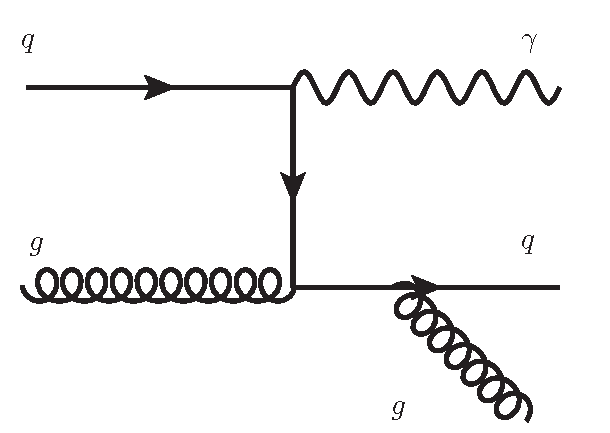
\includegraphics[scale=0.5]{images/Feyn_gjets_compton.pdf}}&
\raisebox{0.0\height}{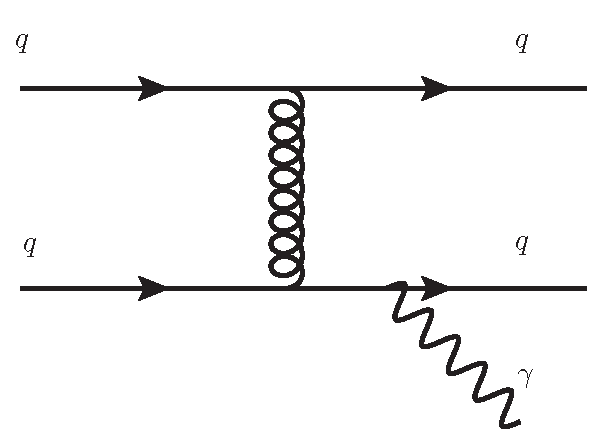
\includegraphics[scale=0.5]{images/gjets_qq2qq_compton.pdf}}
\end{tabular}
}
\subfigure[Bremsstrahlung Radiation]{
\label{fig:SM_pj_brem_copy}
\begin{tabular}{cc}
\raisebox{0.3\height}{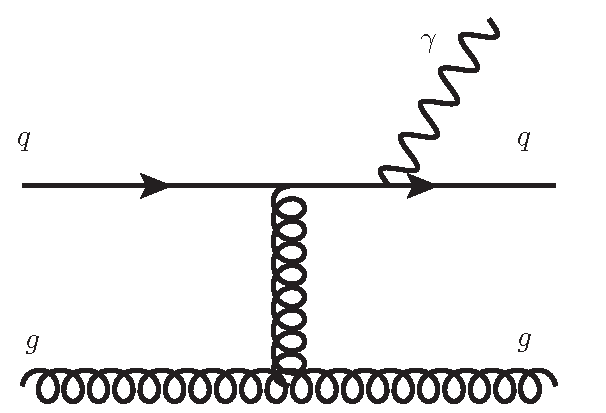
\includegraphics[scale=0.5]{images/Feyn_gjet_brem.pdf}} &
\raisebox{0.0\height}{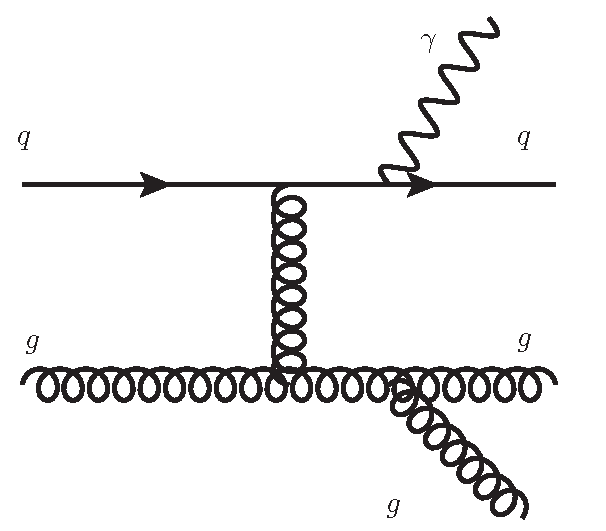
\includegraphics[scale=0.5,keepaspectratio=true]{images/Feyn_gjets_brem.pdf}}
\end{tabular}
}
\end{center}
\caption{Leading-order and next-to-leading-order Feynman diagrams for Standard Model prompt photon production. Next-to-leading-order production will have extra gluon radiation and/or gluon exchanges.}
\label{fig:SM_pj_Feynmans_copy}
\end{figure}


SM prompt $\gamma$ + jets is the largest background for the $\gamma$ + jets signature. It is assumed that SM processes are the only sources of prompt photon + jets; therefore, any excess measured is either from other types of backgrounds or new processes that the SM does not account for. The Feynman diagrams for SM $\gamma$ + jets production are shown in Fig.~\ref{fig:SM_pj_Feynmans_copy}. In the SM, a photon couples to an initial or final-state quark or antiquark. The outgoing quark(s) or gluon(s) is (are) observed as the jet(s). The annihilation of a quark and an antiquark is the dominant production mechanism. Quark and gluon scattering (Compton scattering) is the second largest mechanism (see Table~\ref{tab:gjDiagramsCrossSection}). The third mechanism, termed bremsstrahlung, has a photon radiated off a quark or an antiquark. The bremsstrahlung mechanism is suppressed by the photon isolation requirement and decreases with increasing $p^{\gamma}_{T}$. As there are no undetectable particles present in these processes, any missing transverse energy in the event will be due to mismeasurements of calorimeter energy.

\begin{table}[htbm]
\caption{Cross sections of the two dominant contributions to $\gamma$ + jet production and their contributions to the total cross section.}
\label{tab:gjDiagramsCrossSection}
\centering
\begin{tabular}{cc}
\hline
\BUbf{Diagram} & \BUbf{Cross Section}\\
\hline
 Annihilation ($q + \bar{q}\to g + \gamma$) & 1.8$\time 10^{-3}$ mb (62\%)\\
 Compton ($q + g \to q + \gamma$) & 1.1$\time 10^{-3}$ mb (38\%)\\
\hline
\end{tabular}
\end{table}

SM prompt \phojets production is modeled using \pythiaText Monte Carlo events selected according to the event selection described in Section~\ref{sec:EventSelection} with the exception of the trigger and EM timing requirements. Table~\ref{tab:SMphotonSelection} summarizes the selection criteria.

\begin{table}[h!]
\caption{Event selection requirements to model the SM $\gamma$ background.}
\label{tab:SMphotonSelection}
\centering
 \begin{tabular}{cc}
\hline
\BUbf{Selection Variable} & \BUbf{Requirement}\\
\hline
Goodrun & Pass\\
Trigger & N/A\\
Primary Vertices & $\geq1$ and its $z$ position $|z|<60$~cm\\[2ex]
\sc{Photon Selection} & $E_{T}^{\gamma} > 30$~\etUnits, $|\eta_{detector}^{\gamma}|<1.1$\\
& Pass tight photon selection requirements\\
& (see Table~\ref{tab:tightAndLoosePhotonCuts})\\[2ex]
EM timing & N/A\\
Tracks (Phoenix) & No phoenix tracks\\
Muon stubs & N/A\\
Beam halo selection requirements & N/A\\[2ex]
\sc{Jet Selection} & $\geq$1 jet with $E_{T}^{jet} > 15$~\etUnits, $|\eta_{detector}^{jet}|< 3.0$\\
Jet--\met separation & $\Delta \phi(\met - \mathrm{jet})>0.4$\\
\hline
 \end{tabular}
\end{table}


These Monte Carlo events are weighted according to the number of vertices to match the instantaneous luminosity profile of data. For this, a set of weights is derived by comparing the vertex distribution of \phoonejet events in data to MC. The vertex distribution in data and MC is normalized to unit area and the ratio of data to photon MC is taken. The weight for a photon MC event with $n$ vertices is:

\begin{equation}
W_{n-vtx}^{\gamma+jet} = \frac{X_{n-vtx}^{\mathrm{Data}}}{X_{n-vtx}^{\mathrm{SM} \gamma}}
\label{eqa:phoMCvtxWeights}
\end{equation}

\noindent where $X_{n-vtx}^{\mathrm{Data}}$ is the fraction of data events in the bin with $n$ vertices and $X_{n-vtx}^{\mathrm{SM} \gamma}$ is the fraction of $\gamma$ MC events in the same bin.

After weighting, this sample of events is normalized to the expected number of SM $\gamma$ + jets events ($N^{\mathrm{SM}\gamma}$) to make the final template, as described by Equations~\ref{eqa:SMQCDscaling}, \ref{eqa:FakeFraction}, and \ref{eqa:MtdANorm} in the beginning of \mbox{Method A} (Section \ref{sec:MethodA}).




%%%%%%%%%%%%%%%%%%%%%%%%%%%%%% QCD background
\subsection{QCD Multijet Background}\label{sec:QCDbackground}
The QCD multijet background, in which a jet fakes a prompt photon ($\gamma^{jet\to \gamma}$), is the largest source of fake prompt photons. These are events where jets from light mesons decay into photons. Often, \pizero, $\eta$, and $\rho$ particles are produced and they decay almost exclusively into several photons. The dominant decay modes of \pizero and $\eta$ mesons are shown in Table~\ref{tab:PizeroEtaDecayModes}. As shown in Fig.~\ref{fig:DijetFeynmanDiags}, some of the Feynman diagrams of jet production are very similar to those of prompt photon production, in which the photon is replaced by a quark or a gluon. %And these processes cannot be distinguished and hence this background is irreducible.


\begin{table}[h]
\caption{Dominant decay modes of light mesons (\pizero and $\eta$) as a fraction of the full decay width.}
\label{tab:PizeroEtaDecayModes}
\centering
\begin{tabular}{ccc}
\hline
\BUbf{Meson} & \BUbf{Dominant Decay Modes} & \BUbf{Fraction}\\
\hline
\pizero & 2$\gamma$ & (98.798~$\pm$~0.032)\%\\[1ex]
\multirow{2}{*}{$\eta$} & 2$\gamma$ & (72.0~$\pm$~0.5)\%\\
 & 3\pizero & (39.43~$\pm$~0.26)\%\\
\hline
\end{tabular}
\end{table}


\begin{figure}[h]
 \centering
\subfigure[]
{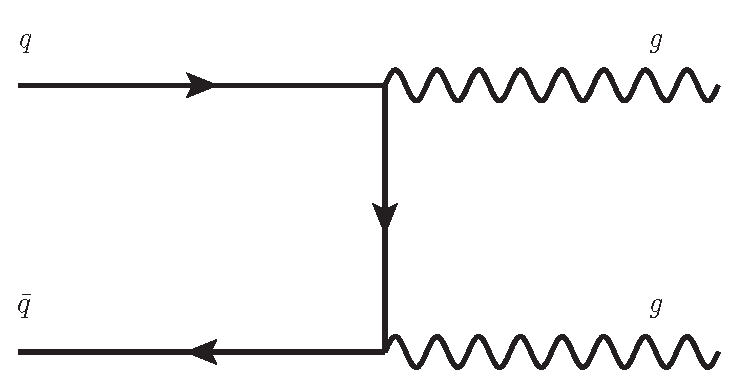
\includegraphics[scale=0.5,keepaspectratio=true]{./Feyn_qqTogg_Annihilation.pdf}
% Feyn_qqTogg_Annihilation.pdf: 354x182 pixel, 72dpi, 12.49x6.42 cm, bb=0 0 354 182
}
\subfigure[]
{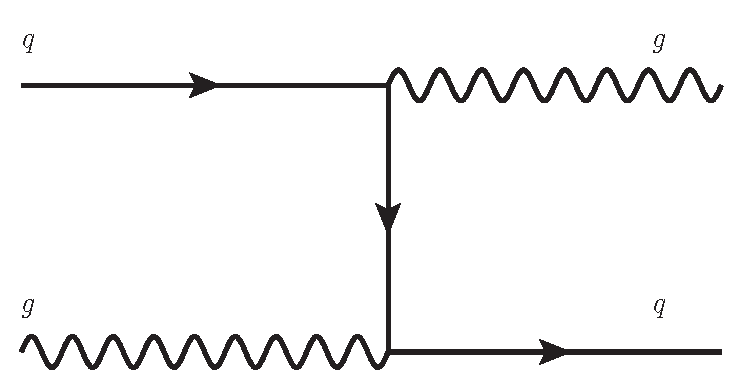
\includegraphics[scale=0.5,keepaspectratio=true]{./Feyn_qgTogq_Compton.pdf}
 % Feyn_qgTogq_Compton.pdf: 355x182 pixel, 72dpi, 12.52x6.42 cm, bb=0 0 355 182
}
 \caption{Feynman diagrams of two of the many dijet production processes in the SM. These jets can decay into neutral mesons that eventually decay into one or more photons. This background is very significant as the dijet production cross section is much larger than that of $\gamma$ + jets.}
 \label{fig:DijetFeynmanDiags}
\end{figure}

If the two photons from \pizero$\to \gamma\gamma$ are not too energetic, the CES detector can be used to resolve them and hence the event can be removed from selection. If the two photons produced are energetic, the CES is not able resolve them and they would be reconstructed as a single photon as illustrated in Fig.~\ref{fig:JetFakingPhoton}. In this case, the hits (ADC counts or the MIPs) in the CPR detector are used to identify and remove such events. The requirements on isolation energy, second CES cluster, and $\chi^{2}$ in photon selection requirements suppress this background significantly. The rate for a jet to fake an isolated photon is about $\sim$10$^{-4}$ at 30~GeV and decreases rapidly with increasing jet energy (see Fig.~\ref{fig:JetFakeRate}). Still, the QCD multijet background is a significant source of fake photons as the jet production cross section is significantly larger than $\gamma$ production.

\begin{figure}[p]
 \centering
 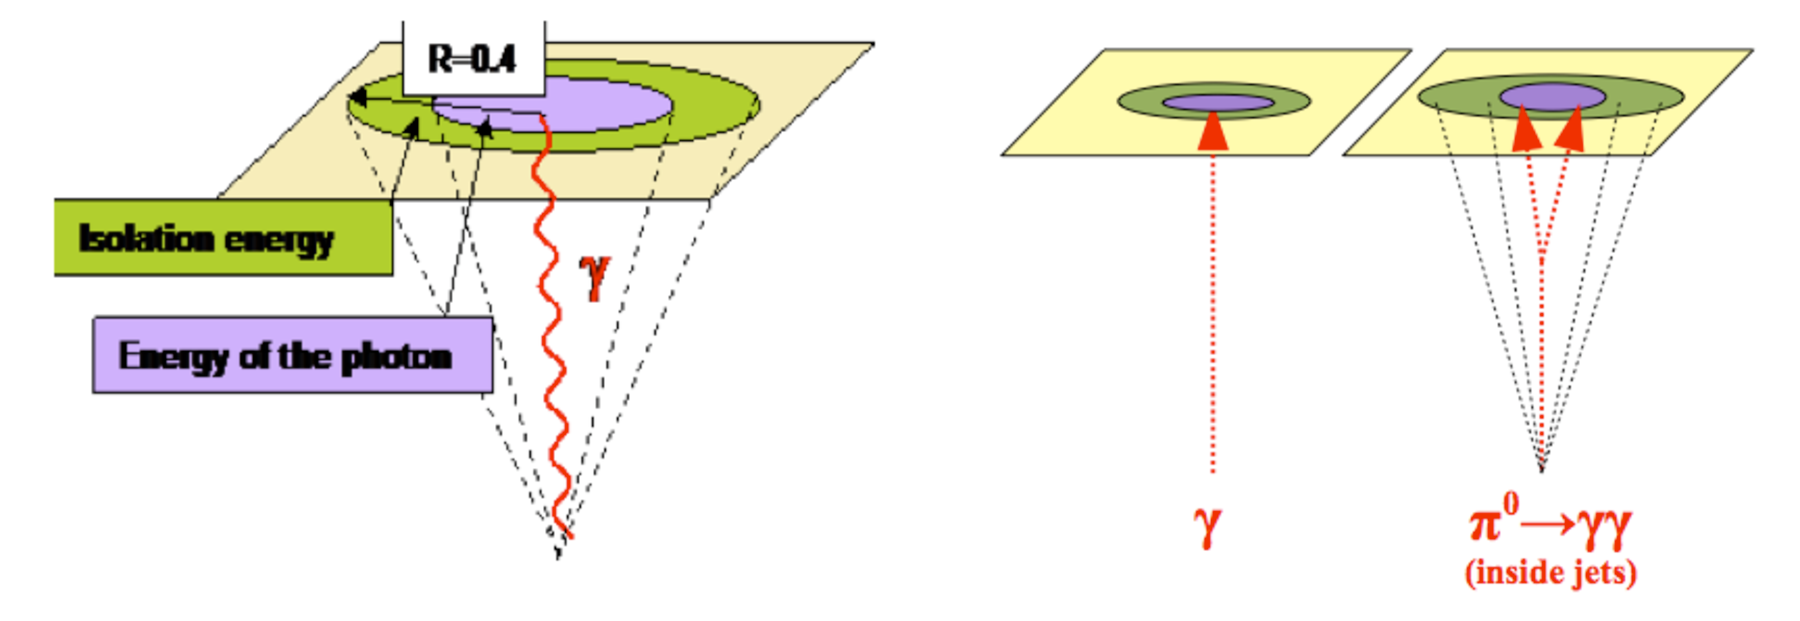
\includegraphics[scale=0.5,keepaspectratio=true]{./JetFakingPhotonIllustration.pdf}
 % JetFakingPhotonIllustration.pdf: 864x298 pixel, 72dpi, 30.48x10.51 cm, bb=0 0 864 298
 \caption{Reconstruction of a single photon in the detector (left). Energetic photons from light meson decay are identified as a single photon by the CES detector (right).}
 \label{fig:JetFakingPhoton}
\end{figure}


\begin{figure}[p]
\begin{center}
 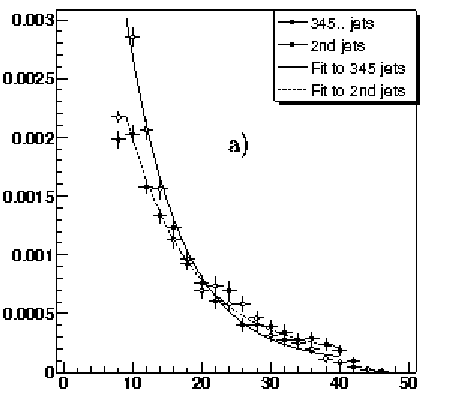
\includegraphics[scale=1.6,keepaspectratio=true]{./JetFakeRate.pdf}
 % JetFakeRate.pdf: 612x792 pixel, 72dpi, 21.59x27.94 cm, bb=0 0 612 792
 \caption{Probability of a jet faking an isolated photon as studied using Monte Carlo events. The rate decreases rapidly with increasing \et of the jet \cite{cdfnote:6363}.}
 \label{fig:JetFakeRate}
\end{center}
\end{figure}

This background is modeled using a sample of events selected from data. Events with a photon candidate that passes loose photon selection requirements, but does not pass tight photon selection requirements, are selected. These photons are referred to as \newterm{sideband photons}. Most of the fake jets in data selected using tight photon selection requirements are from quarks, whereas the sideband photons are mostly gluons. The isolation energy requirement strongly discriminates between the two samples. This is because of the extra color carried by the gluons, which creates extra particles in a larger region of the detector; thereby causing a failure of the isolation requirement in the tight photon ID requirements. The selection criteria used to select these events (\newterm{sideband events}) are listed in Table~\ref{tab:SidebandSelection}.


\begin{table}[htmb!]
\caption{Sideband event selection requirements to model the QCD multijet background.}
\label{tab:SidebandSelection}
\centering
 \begin{tabular}{cc}
\hline
\BUbf{Selection Variable} & \BUbf{Requirement}\\
\hline
Goodrun & Pass\\[1ex]
\multirow{2}{*}{Trigger} & Pass any one of the triggers\\
& \firstphotrig, \secondphotrig, \thirdphotrig \\[1ex]
Primary Vertices & $\geq$1 and its $z$ position $|z|<60$~cm\\[2ex]
\sc{Photon Selection} & $E_{T}^{\gamma} > 30$~\etUnits, $|\eta_{detector}^{\gamma}|<1.1$\\
& Pass loose photon selection\\
& requirements but fail tight photon\\
& selection requirements (see Table~\ref{tab:tightAndLoosePhotonCuts})\\[2ex]
EM timing & $|\Delta t^{\gamma}|<4.8$~ns\\
Tracks (Phoenix) & No phoenix tracks\\
Muon stubs & 0 (No muon stubs)\\
Beam halo selection requirements & Fail\\[2ex]
\sc{Jet Selection} & $\geq$1 jet with $E_{T}^{jet} > 15$~\etUnits, $|\eta_{detector}^{jet}|< 3.0$\\
Jet--\met separation & $\Delta \phi(\met - \mathrm{jet})>0.4$\\
\hline
 \end{tabular}
\end{table}

The expected number of QCD events ($N^\mathrm{QCD}$) is determined using equations \ref{eqa:SMQCDscaling}, \ref{eqa:FakeFraction}, and \ref{eqa:MtdANorm} as described in the beginning of this section. There is a fraction of electroweak, beam halo, and cosmic ray events present in the sideband sample. These events are subtracted prior to scaling to avoid the counting of such events twice.

%%%%%%%%%%%%%%%%%%%%%%%%%%%%%% Lepton+Jets background
\subsection{Electroweak Background}\label{sec:elejets}
The electroweak background is mainly from $W$, $Z$, $WW$, $WZ$, and $ZZ$ production, in which a lepton emits a photon as collinear final-state radiation or hard bremsstrahlung as it traverses the detector material, and that photon is identified as the prompt photon ($\gamma^{e\to \gamma}$). Most of these leptons come from $W$ decay to leptons. Less significant contributions come from $Z$ and di-boson decay to leptons. The fake probability decreases rapidly with the increasing energy of the lepton.

A small portion of the electroweak background comes from a failure to reconstruct the associated track of a lepton due to inefficiencies in track reconstruction. Partial tracks of such leptons are traced and matched using outside-in track reconstruction. This algorithm tries to find a calorimeter energy deposition with hits in the silicon detector and COT, and this is known as \newterm{Phoenix} track reconstruction for historical reasons \cite{pap:PhoenixTracking}. The Phoenix track-finding algorithm is about 60\% effective in rejecting leptons with energies \etg{30}. Electron candidates with Phoenix tracks are removed from the selection. The probability of a remaining electron candidate faking a photon decreases rapidly as the electron energy increases, as shown in Fig.~\ref{fig:ElectronFakeRate} \cite{cdfnote:8220}. The fake rate is $<0.007$ for an electron with \etg{30}.

\begin{figure}
\begin{center}
 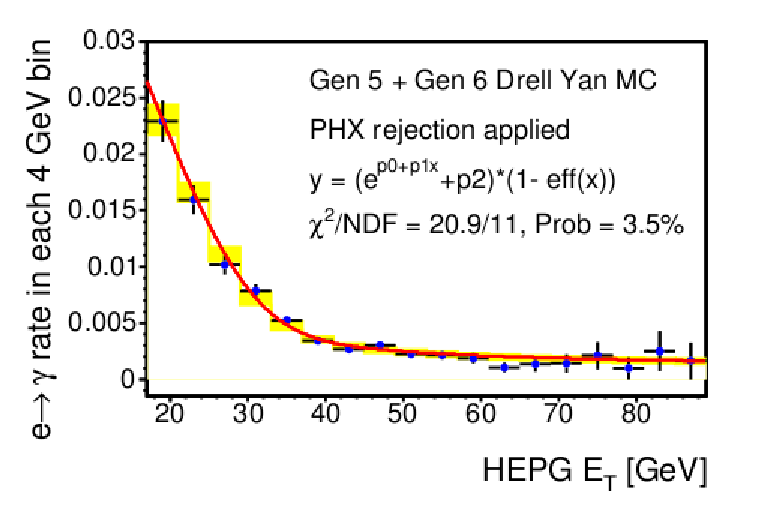
\includegraphics[scale=0.9]{./EleFakeRate.pdf}
 % EleFakeRate.pdf: 367x248 pixel, 72dpi, 12.95x8.75 cm, bb=0 0 367 248
\caption{Probability for a tight central electron to fake a tight photon as a function of the \et of the generator-level electron. The reference curve indicates the fake rate function fitted to the data and the yellow shaded area indicates the systematic uncertainty.}
\label{fig:ElectronFakeRate}
\end{center}
\end{figure}


The distribution of the remaining \elejets events is modeled using electroweak Monte Carlo data generated using \pythiaText. The event selection is summarized in Table~\ref{tab:EWKSelection}.

\begin{table}[htmb!]
\caption{Event selection requirements for modeling the SM electroweak background.}
\label{tab:EWKSelection}
\centering
 \begin{tabular}{cc}
\hline
\BUbf{Selection Variable} & \BUbf{Requirement}\\
\hline
Goodrun & Pass\\
Trigger & N/A\\
Primary Vertices & $\geq$1 with $|z|<60$~cm\\[2ex]
\sc{Photon Selection} & $E_{T}^{\gamma} > 30$~\etUnits, $|\eta_{detector}^{\gamma}|<1.1$\\
& Pass tight photon selection requirements\\
& (see Table~\ref{tab:tightAndLoosePhotonCuts})\\[2ex]
EM timing & N/A\\
Tracks (Phoenix) & No phoenix tracks\\
Muon stubs & N/A\\
Beam halo selection requirements & N/A\\[2ex]
\sc{Jet Selection} & $\geq$1 jet with $E_{T}^{jet} > 15$~\etUnits, $|\eta_{detector}^{jet}|< 3.0$\\
Jet--\met separation & $\Delta \phi(\met - \mathrm{jet})>0.4$\\
\hline
 \end{tabular}
\end{table}

Events satisfying the criteria in Table~\ref{tab:EWKSelection} are selected from individual MC samples: \zee, \zmm, \ztt, \wen, \wmn, and \wtn. These events are corrected for multiple interactions and the underlying event as described below. The same MC samples are used to select \wjets and \zjets events and are compared to the corresponding events measured in data.

% \addtolength{\parskip}{\baselineskip}
\subsubsection{Corrections to $W$ MC Events}\label{sec:ewkWMCcorrections}
The selected $W$ MC events are corrected to match the instantaneous luminosity profile of the data. Corrections for these events are derived to accurately model the underlying event and multiple interactions.

To correct for multiple interactions, a set of weights is derived as a function of the number of vertices ($N_{vtx}$) by comparing $W$ + jets events in data to Monte Carlo events.

In generating weights for $W$ events, an electron candidate is first identified using the photon-like electron selection requirements (see Table~\ref{tab:pecuts}). Then, the event is required to have \metg{20} to account for the $\nu$ which escapes detection. From this the $W$ is reconstructed. To reduce the background for $W$ selection, a standard selection requirement on the transverse mass is applied. Finally, one or more jets is required with \etg{15}. The selection of $W$+ jets events is summarized in Table~\ref{tab:WJetSelection}.

\begin{table}[htmb!]
\caption{$W$ + jets event selection requirements to correct for multiple interactions and the underlying event in \wen, \wmn, and \wtn MC events.}
\label{tab:WJetSelection}
\centering
 \begin{tabular}{cc}
\hline
\BUbf{Selection Variable} & \BUbf{Requirement}\\
\hline
Goodrun & Pass\\
Trigger & N/A\\
Primary Vertices & $\geq$1 with $|z|<60$~cm\\[2ex]
\sc{Electron Selection} & $E_{T}^{e} > 20$~\etUnits, $|\eta_{detector}^{e}|<1.1$\\
& Pass tight photon-like electron selection requirements\\
& (see Table~\ref{tab:pecuts})\\[2ex]
EM timing & N/A\\
\met \sc{Selection}& \met$>20$~\etUnits\\[2ex]
\sc{Reconstructed} $W$ & $E_{T}^{W} > 30$~\etUnits, $|\eta_{detector}^{W}|<1.1$\\
(from $e$ and \met) & transverse mass $60<M_{T}^{W}<100~$\massunits\\[2ex]
\sc{Jet Selection} & $\geq$1 jet with $E_{T}^{jet} > 15$~\etUnits, $|\eta_{detector}^{jet}|< 3.0$\\
Jet--\met separation & $\Delta \phi(\met - \mathrm{jet})>0.4$\\
\hline
 \end{tabular}
\end{table}

The basis for this $W$ + jet selection is to use the $W$ boson to represent the leading photon, hence the selection requirements on \pt and $\eta$ are identical. The vertex and \met distributions in \wjets data and \MC are compared. The vertex distributions are normalized to unity and then the data to \MC ratio is taken. After weighting the MC sample with vertex weights ($W_{vtx}^{W+jets}$), the \met distribution is normalized according to the integrated luminosity of the data, and the data to \MC ratio is taken (see Figs.~\ref{fig:WJets_NvtxWgts} and \ref{fig:WJets_MetWgts}). The \met weights ($W_{\met}^{W+jets}$) are derived in bins of \met and applied where possible. The same vertex and \met weights are used to reweight all the $W$ \MC samples. The total weight for a $W$ MC event is:

\begin{equation}
 W^{W+jets} = W_{vtx}^{W+jets} \times W_{\met}^{W+jets} = \frac{N^{W+jets~Data}_{vtx}}{N^{W+jets~MC}_{vtx}} \times \frac{\met^{W+jets~Data}}{\met^{W+jets~MC}}
 \label{eqa:WjetsWeights}
\end{equation}
The distribution of weights is shown in Fig.~\ref{fig:WJets_NvtxWgts} and Fig.~\ref{fig:WJets_MetWgts}.

\begin{figure}[p]
 \centering
 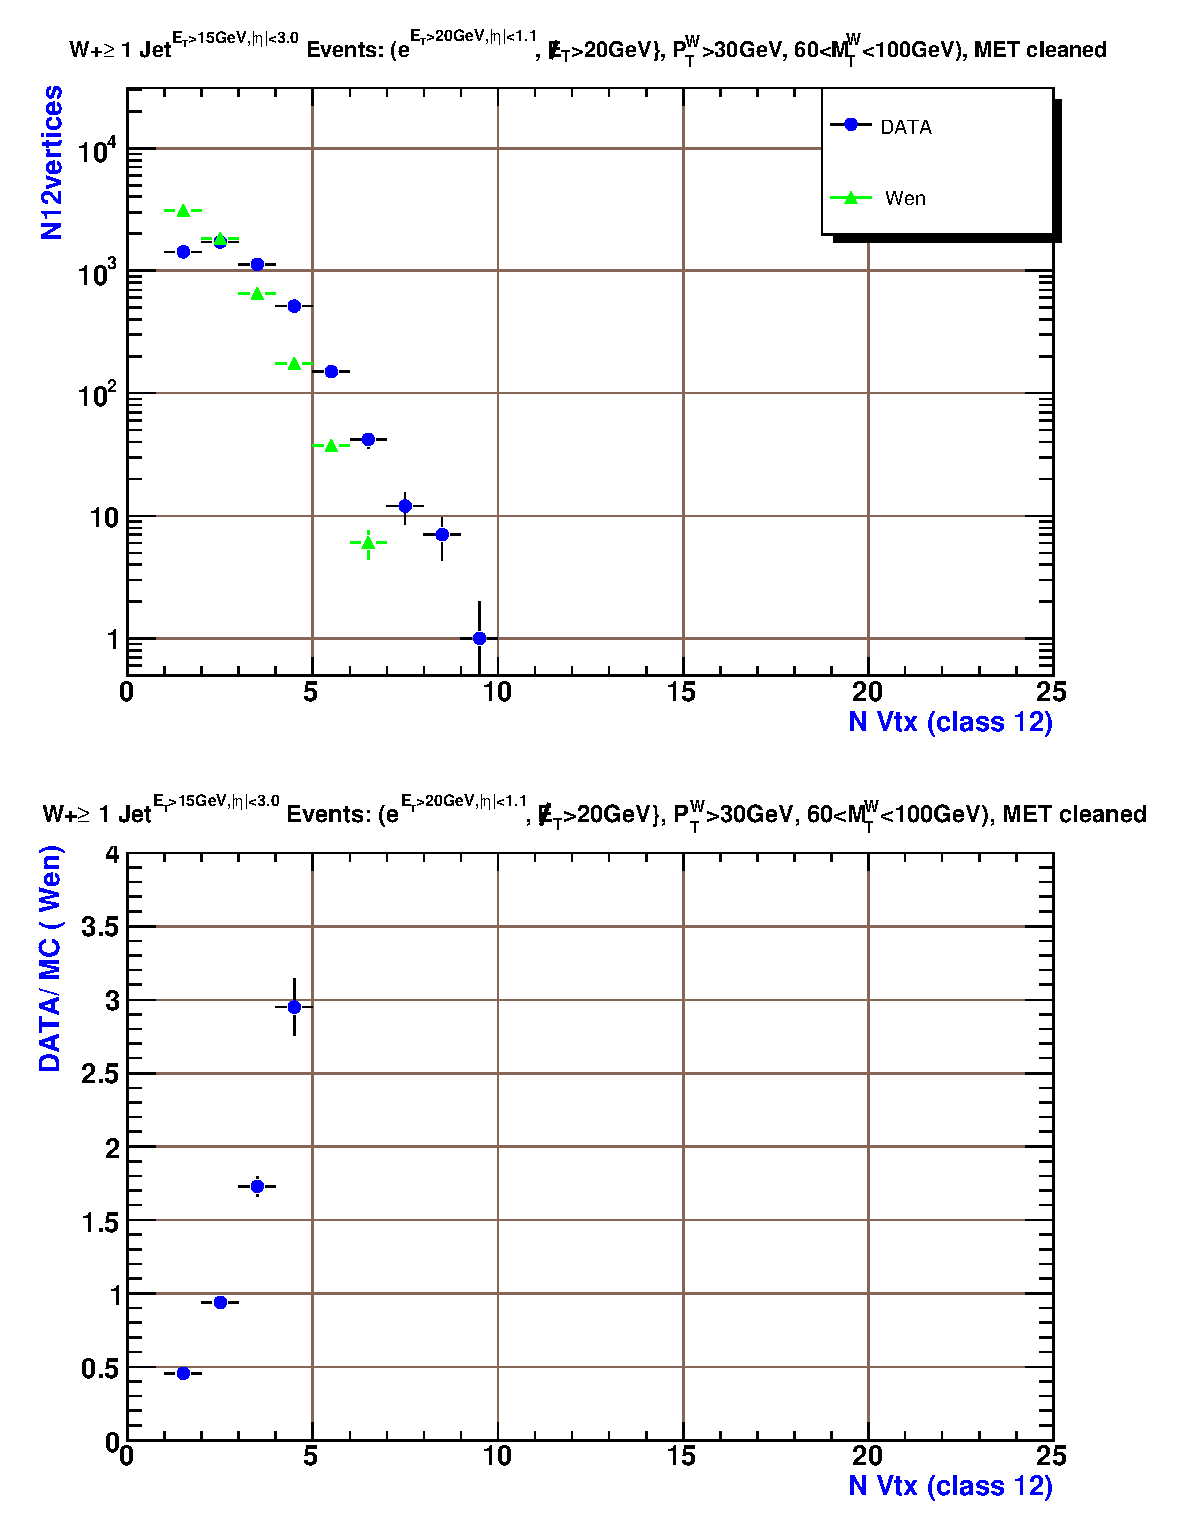
\includegraphics[scale=0.8,keepaspectratio=true]{./WJets_NvtxWgts.pdf}
 % WJets_NvtxWgts.pdf: 567x734 pixel, 72dpi, 20.00x25.89 cm, bb=0 0 567 734
 \caption{Distribution of the number of vertices in $W$+ jets data and MC events prior to weighting the MC events. The top plot shows the distribution with a logarithmic scale. The bottom plot is the ratio of Data to MC, which shows the actual weights used in the weighting process.}
\label{fig:WJets_NvtxWgts}
\end{figure}

\begin{figure}[p]
 \centering
 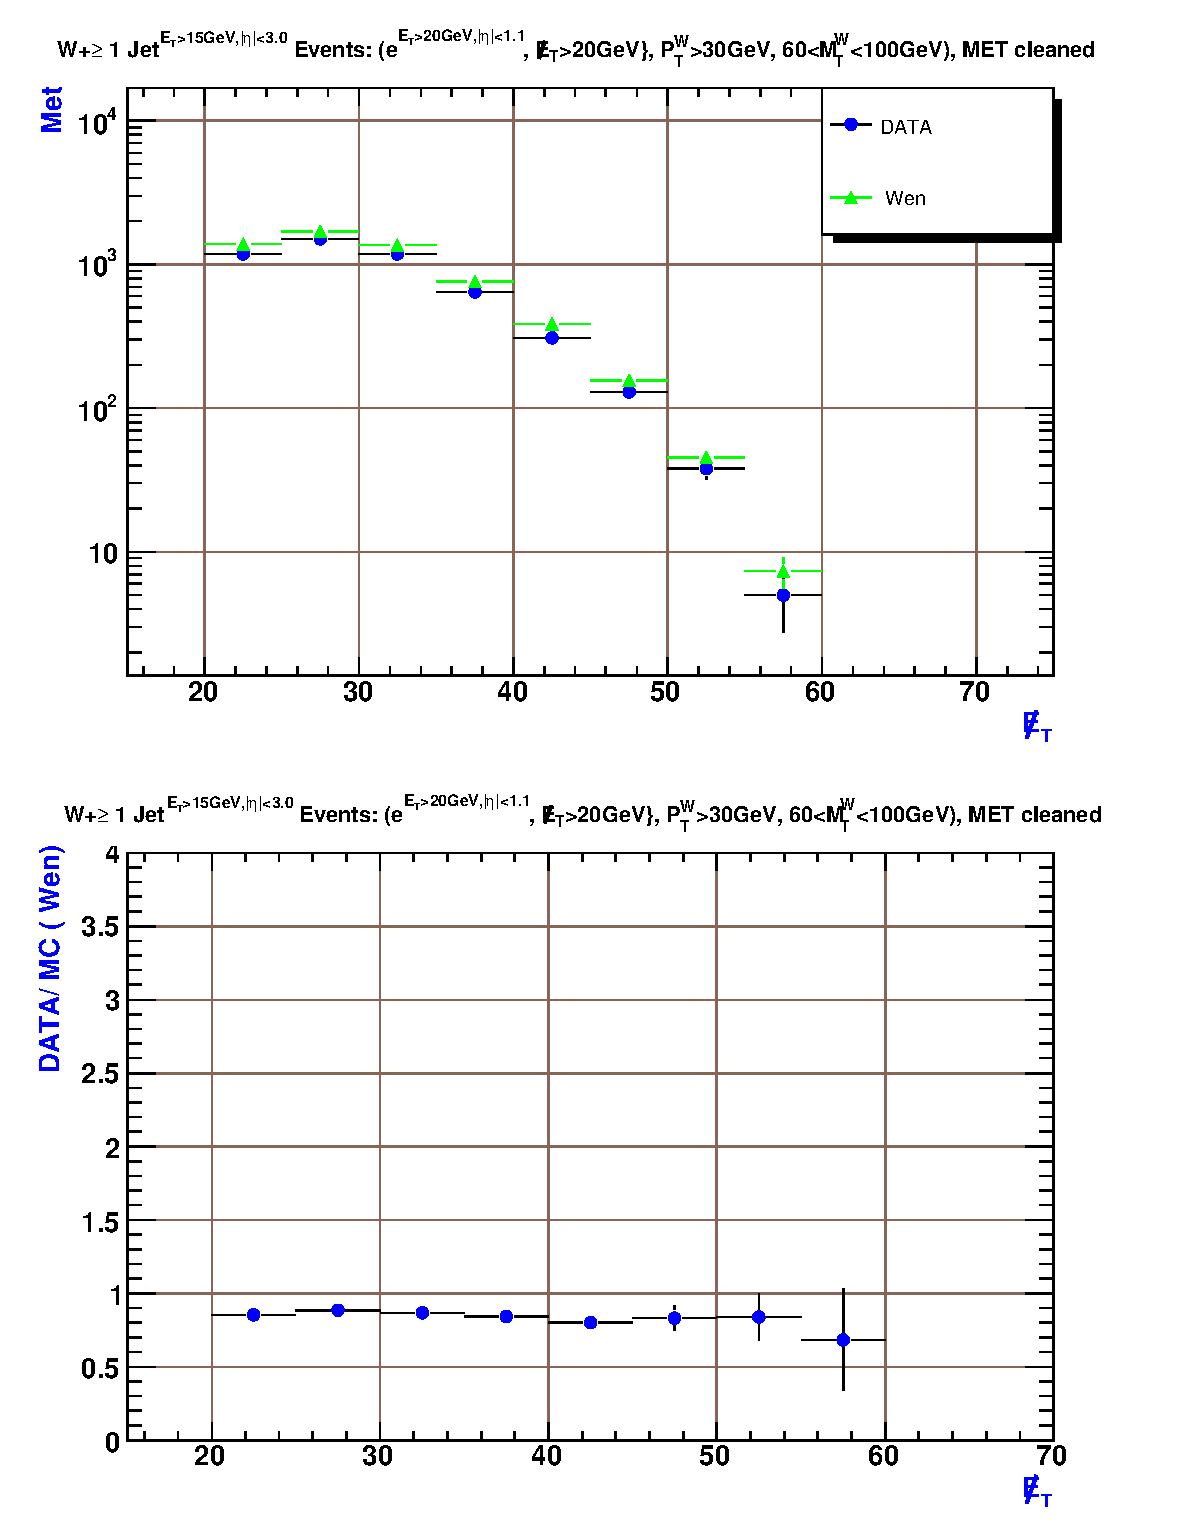
\includegraphics[scale=0.8,keepaspectratio=true]{./WJets_MetWgts.pdf}
 % WJets_NvtxWgts.pdf: 567x734 pixel, 72dpi, 20.00x25.89 cm, bb=0 0 567 734
 \caption{Distribution of the \met in $W$+ jets data and MC events prior to weighting the MC events. The top plot shows the distribution with a logarithmic scale. The bottom plot is the ratio of Data to MC, which shows the actual weights used in the weighting process.} \label{fig:WJets_MetWgts}
\end{figure}

\subsubsection{Corrections to $Z$ MC Events}\label{sec:ewkZMCcorrections}
Similarly, \zjets events are selected according to the selection criteria in Table~\ref{tab:ZJetSelection} and weights are generated by comparing data to \MC events. \zjets events are corrected only for multiple interactions by comparing vertex distributions. The underlying event corrections could not be derived due to limited statistics.

\begin{table}[htmb!]
\caption{$Z$ + jets event selection requirements to correct for multiple interactions in \zee, \zmm, and \ztt MC events.}
\label{tab:ZJetSelection}
\centering
 \begin{tabular}{cc}
\hline
\BUbf{Selection Variable} & \BUbf{Requirement}\\
\hline
Goodrun & Pass\\
Trigger & N/A\\
Primary Vertices & $\geq$1 and its $z$ position $|z|<60$~cm\\[2ex]
\sc{Electrons Selection} & $E_{T}^{e} > 20$~\etUnits\\
& One of the two must be in $|\eta_{detector}^{e}|<1.1$\\
& \& the other can be in $|\eta_{detector}^{e}|<3.0$\\
& Both electrons pass tight\\
& photon-like electron selection\\
& requirements(see Table~\ref{tab:pecuts})\\[2ex]
EM timing & N/A\\[2ex]
\sc{Reconstructed} $Z$ & $E_{T}^{Z} > 30$~\etUnits, $|\eta_{detector}^{Z}|<1.1$\\
(from $e$ and \met) & $76<M_{Z}<106$~\massunits\\[2ex]

\sc{Jet Selection} & $\geq$1 jet with $E_{T}^{jet} > 15$~\etUnits, $|\eta_{detector}^{jet}|< 3.0$\\
Jet--\met separation & $\Delta \phi(\met - \mathrm{jet})>0.4$\\
\hline
 \end{tabular}
\end{table}

The total weight for an event in the $Z$ MC sample is:

\begin{equation}
 W^{Z+jets}_{vtx}= \frac{N^{Z+jets~Data}_{vtx}}{N^{Z+jets~MC}_{vtx}}
 \label{eqa:ZjetsWeights}
\end{equation}

The calculation of the expected number of electroweak events from each individual decay mode is listed below. Here, $X_{i}$ denotes a measurement from a qualifying event.

\begin{eqnarray}
N^{W\to e\nu} &=& \frac{{\cal L}^{Data}}{{\cal L}^{W\to e\nu}} \sum_{i} X_{i} \cdot W^{vtx(W+jets)}_{i} \cdot W^{\sla{E}_{T}(W+jets)}_{i}\\
N^{W\to \mu\nu} &=& \frac{{\cal L}^{Data}}{{\cal L}^{W\to \mu\nu}} \sum_{i} X_{i} \cdot W^{vtx(W+jets)}_{i} \cdot W^{\sla{E}_{T}(W+jets)}_{i}\\
N^{W\to \tau\nu} &=& \frac{{\cal L}^{Data}}{{\cal L}^{W\to \tau\nu}} \sum_{i} X_{i} \cdot W^{vtx(W+jets)}_{i} \cdot W^{\sla{E}_{T}(W+jets)}_{i}\\
N^{Z\to ee} &=& \frac{{\cal L}^{Data}}{{\cal L}^{Z\to ee}} \sum_{i} X_{i} \cdot W^{vtx(Z+jets)}_{i}\\
N^{Z\to \mu\mu} &=& \frac{{\cal L}^{Data}}{{\cal L}^{Z\to \mu\mu}} \sum_{i} X_{i} \cdot W^{vtx(Z+jets)}_{i}\\
N^{Z\to \tau\tau} &=& \frac{{\cal L}^{Data}}{{\cal L}^{Z\to \tau\tau}} \sum_{i} X_{i} \cdot W^{vtx(Z+jets)}_{i}
\label{eqa:WenTotal}
\end{eqnarray}
The total electroweak background with all corrections is defined using:
\begin{equation}
N^{EWK} = N^{W\to e\nu} + N^{W\to \mu\nu} + N^{W\to \tau\nu} + N^{Z\to ee} + N^{Z\to \mu\mu} + N^{Z\to \tau\tau}
\label{eqa:EWKtotalWeighted}
\end{equation}



%%%%%%%%%%%%%%%%%%%%%%%%%%%%%%%%%%%%%%%%%%%%%%%%%%%%%%%%%%%%%%%%%%%%%
%            di-photon background
%%%%%%%%%%%%%%%%%%%%%%%%%%%%%%%%%%%%%%%%%%%%%%%%%%%%%%%%%%%%%%%%%%%%%
\subsection{Di-photon Background}\label{sec:diphoton}

This is a SM process in which a pair of photons is produced in the primary collision. The production mechanism is different from SM \phojets as shown by the Feynman diagrams in Fig.~\ref{fig:Feyn_dipho_annihilation}. But the processes are difficult to distinguish from one another due to the way the $\gamma$ + jet events are selected. One of the photons produced will be identified as a prompt photon candidate, and the second photon will be identified as a jet to make the $\gamma$ + jet signature. Although the cross section is smaller by orders of magnitude, the importance of this background is the higher probability to completely lose one of the photons into an uninstrumented region of the detector. About 15\% of the CDF detector is uninstrumented. Hence, the rate of losing one of the photons in an uninstrumented region of the detector is twice as large as in a $\gamma$ + jet event. If a photon is lost in a crack, that event would most likely to appear as a high \met event. This high \met region is exactly where new, undetectable particles are expected.
\begin{figure}[hbtm]
 \centering
 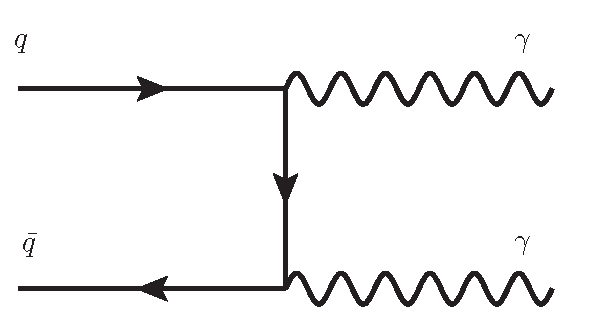
\includegraphics[scale=0.7,keepaspectratio=true]{./Feyn_dipho_annihilation.pdf}
 % Feyn_dipho_annihilation.pdf: 289x151 pixel, 72dpi, 10.20x5.33 cm, bb=0 0 289 151
 \caption{Feynman diagram describing diphoton production in the SM.}
\label{fig:Feyn_dipho_annihilation}
\end{figure}
\vspace{-0.01\textheight}


The distribution of events from this background is modeled using diphoton Monte Carlo data. The event selection is summarized in Table~\ref{tab:DiphoSelection}.

\begin{table}[h!]
\caption{Event selection requirements to model SM the Di-$\gamma$ background.}
\label{tab:DiphoSelection}
\centering
 \begin{tabular}{cc}
\hline
\BUbf{Selection Variable} & \BUbf{Requirement}\\
\hline
Goodrun & Pass\\
Trigger & N/A\\
Primary Vertices & $\geq$1 with $|z|<60$~cm\\[2ex]
\sc{Photon Selection} & $E_{T}^{\gamma} > 30$~\etUnits, $|\eta_{detector}^{\gamma}|<1.1$\\
& Pass tight photon selection requirements\\
& (see Table~\ref{tab:tightAndLoosePhotonCuts})\\[2ex]
EM timing & N/A\\
Tracks (Phoenix) & No phoenix tracks\\
Muon stubs & N/A\\
Beam halo selection requirements & N/A\\[2ex]
\sc{Jet Selection} & $\geq$1 jet with $E_{T}^{jet} > 15$~\etUnits, $|\eta_{detector}^{jet}|< 3.0$\\
Jet--\met separation & $\Delta \phi(\met - \mathrm{jet})>0.4$\\
\hline
 \end{tabular}
\end{table}

The selected events are corrected to match the instantaneous luminosity profile of data. The vertex distribution of diphoton events is compared and adjusted to match the vertex distribution in photon + jets data.

Finally, the SM expectation is derived by scaling these events to the integrated luminosity of data. The final prediction for the diphoton background is described by the equation:
\begin{eqnarray}
N^{Di-\gamma} = \frac{{\cal L}^{Data}}{{\cal L}^{Di-\gamma}} \sum_{i} X_{i} \cdot W^{vtx(\gamma+jets)}_{i}
\label{eqa:diPhoFinal}
\end{eqnarray}

%%%%%%%%%%%%%%%%%%%%%%%%%%%%%%%%%%%%%%%%%%%%%%%%%%%%%%%%%%%%%%%%%%%%%
%     NON COLLISION BACKGROUNDS
%%%%%%%%%%%%%%%%%%%%%%%%%%%%%%%%%%%%%%%%%%%%%%%%%%%%%%%%%%%%%%%%%%%%%
\subsection{Non-collision Backgrounds}\label{noncollision_backgrounds}
In addition to the SM backgrounds, there are several other sources that can produce fake photons in the detector. They are photomultiplier tube spikes, beam halo photons, and cosmic photons. Although these are relatively small backgrounds, they tend to populate the large missing energy region and need to be handled carefully.

\subsubsection{PMT Spike Removal}\label{pmtspikes}
Photomultiplier tube (PMT) spikes are a source of a non-collision background caused by a misbehavior of the electronics used to read out the calorimeter. A photomultiplier tube used to readout the calorimeter can produce a signal at random (called a PMT spike). The effect of this is twofold. A PMT spike could manifest itself as a prompt photon from the primary hard scatter. Also, it could lead to a large \met as there is nothing to balance this extra energy.

In the central region of the detector, each calorimeter tower is equipped with two phototubes on either side of the calorimeter for readout. If one of the phototubes has an energy reading, and there is no reading from the other, it is a good indication of a PMT spike. The ``spike killer'' software program will automatically remove events with zero $\sqrt{E_{PMT1}\times E_{PMT2}}$ if there are no soft particles and only PMT noise is found. ($E_{PMT1}$ and $E_{PMT2}$ are the energy readings from the two phototubes, respectively.) Such PMT-spike events are further removed by calculating the asymmetry of the energy readings of the two phototubes, as defined by
\begin{equation}
\mathrm{PMT~Asymmetry} = \frac{E^{PMT1} - E^{PMT2}}{E^{PMT1} + E^{PMT2}}.
\label{eqa_PMTAsymmetry}
\end{equation}
In every event, the PMT asymmetry is measured in both EM and HAD calorimeters (see Fig.~\ref{fig_PMTAsymmetry}). Events with any EM calorimeter tower with $\mathrm{|PMT~Asymmetry}| > 0.65$ or HAD calorimeter tower with $\mathrm{|PMT~Asymmetry}| > 0.85$ \cite{cdfnote:9184} are removed from the event selection. These selection requirements effectively remove 100\% of these fake photon events without removing any true photon events \cite{cdfnote:7960}.

\begin{figure}[hbtm]
\begin{centering}
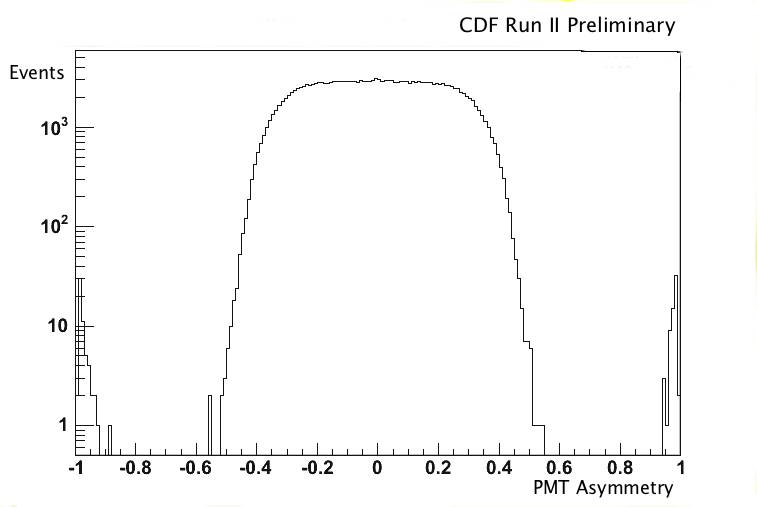
\includegraphics[scale=0.37]{PMT_EM_Asym_twrE_gt_10.jpg}
\caption[PMT Asymmetry.]{PMT Asymmetry observed from EM calorimeter towers with \mbox{$E>10$}~\etUnits. The clumps at the extremes indicate PMT spikes.}
\label{fig_PMTAsymmetry}
\end{centering}
\end{figure}

%%%%%%%%%%%%%%%%%%%%%%%%%%%%%%%%%%%%%%%%%%%%%%%%%%%%%%%%%%%%%%%%%%%%%
%     BEAM HALO PHOTON BACKGROUND
%%%%%%%%%%%%%%%%%%%%%%%%%%%%%%%%%%%%%%%%%%%%%%%%%%%%%%%%%%%%%%%%%%%%%
\subsubsection{Beam Halo Photons}\label{halojets}
Background from the beam halo is a non-collision background that happens to overlap with a primary proton-antiproton collision. The protons and antiprotons that are not coalesced, upon hitting the beam pipe, create a miniature shower. Only the muons ($\mu$) survive to make it through the beam pipe. These muons (dubbed ``beam halo'') travel parallel to the beam and interact with the plug and central calorimeters (see Fig.~\ref{fig:beamHaloPath}). Such an EM cluster would pass the photon selection requirements (see Table~\ref{tab:tightAndLoosePhotonCuts}) and make it look like a prompt photon from the primary collision. It is observed that these muons tend to occupy calorimeter $\phi$ wedges 0 and 23 of the CDF detector due the teardrop shape of the colliding beam. The CDF detector experiences more halo events in the directions of incoming protons as the D\O~detector acts as a filter for the halo originating from antiprotons.

\begin{figure}[htbm]
 \centering
 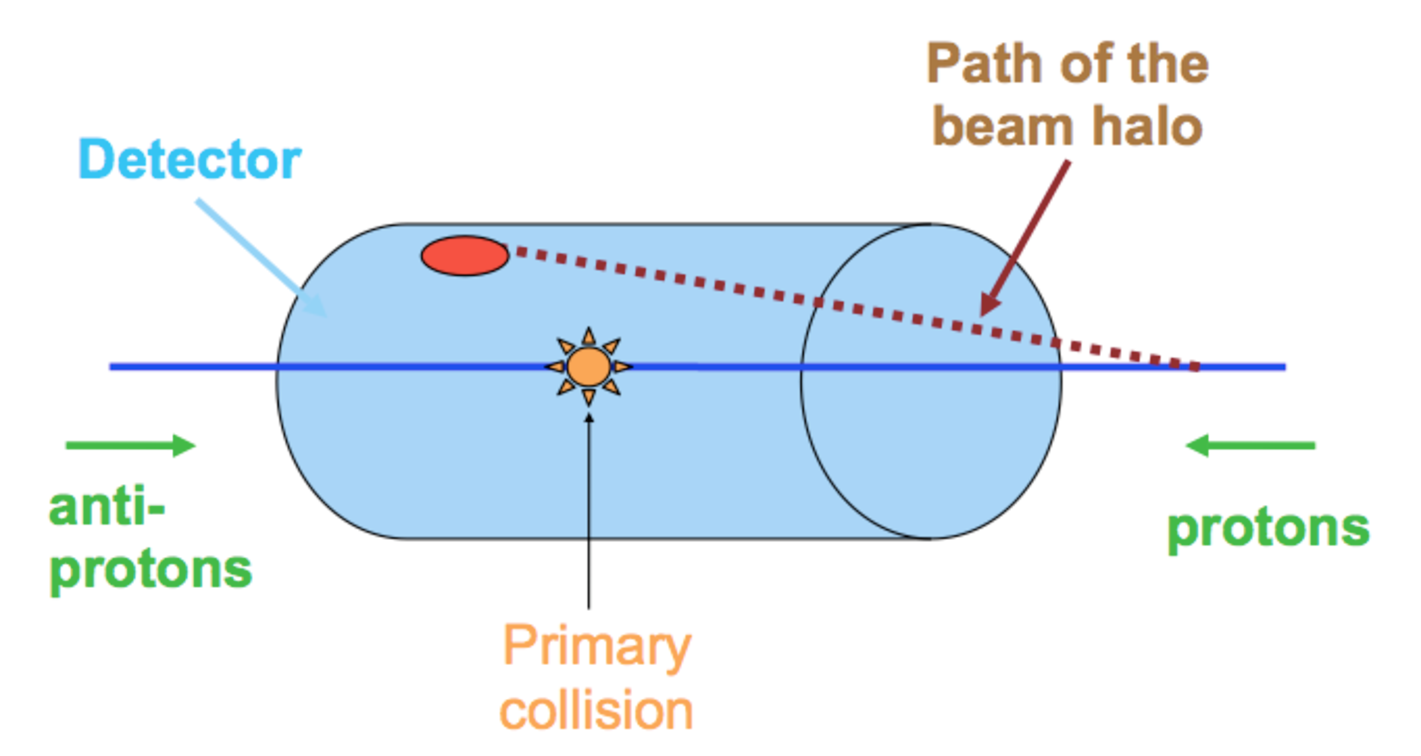
\includegraphics[scale=0.65]{./beam_halo_path.pdf}
 % beam_halo_path.pdf: 682x363 pixel, 72dpi, 24.06x12.81 cm, bb=0 0 682 363
 \caption{Path of the beam halo.}
 \label{fig:beamHaloPath}
\end{figure}

A combination of EM timing and topological selection requirements (see Table \ref{tab:halocuts}) that are orthogonal to the photon selection requirements (see Table~\ref{tab:tightAndLoosePhotonCuts}) are used to identify and remove events with a beam halo photon candidate \cite{ cdfnote:7960, cdfnote:8409}. Figure~\ref{fig:BeamHalo_Identification} shows the beam halo photon candidates isolated by the beam halo selection requirements. Fig.~\ref{fig:CosmicBeamHaloEMtiming} shows the arrival times of the beam halo and cosmic photon candidates at the EM calorimeter.


%%%%%%%%%%%%%%%%%%%% Halo selection requirements %%%%%%%%%%%%%
\begin{table}[p]
\caption{Beam halo selection requirements. The quantity \cutVar{seedWedge} is defined as number of EM towers (\et~$>$~0.1 \etUnits) in the same wedge as the $\gamma$, and \cutVar{Nhad} is defined as the number of plug HAD towers (\et~$>$~0.1 \etUnits) in the same wedge as the $\gamma$. These selection requirements are orthogonal to the photon selection requirements.}
\label{tab:halocuts}
\centering
\begin{tabular} {cc}
\hline
\BUbf{Selection Variable} & \BUbf{Requirement} \\
\hline
\cutVar{seedWedge} & $>$ 8 \\
\cutVar{Nhad} & $>$ 3\\
\hline
\end{tabular}
\end{table}
%%%%%%%%%%%%%%%%%%%%%%%%%%%%%%%%%%%%%%%%%%%
\begin{figure}[p]
 \centering
 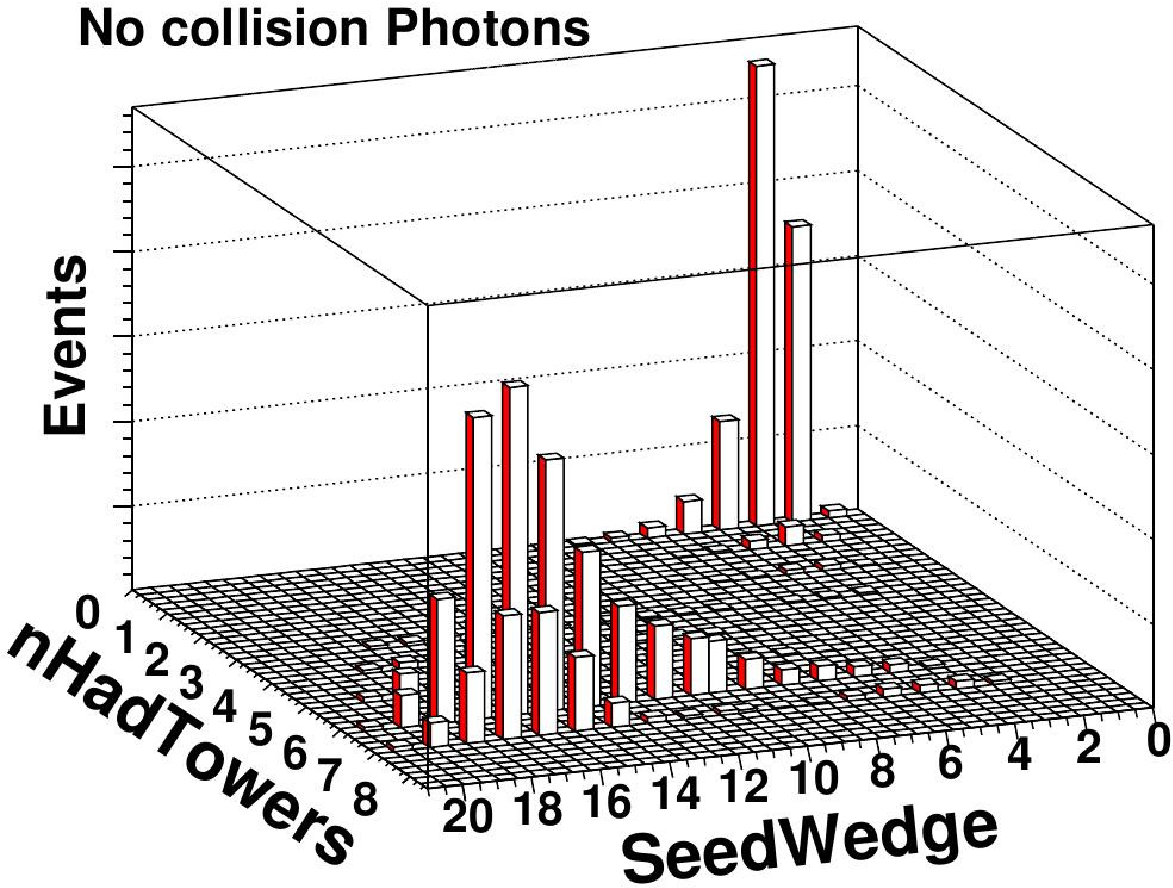
\includegraphics[scale=0.7]{BeamHalo_Topology.pdf}
 % BeamHalo_Topology.pdf: 612x792 pixel, 72dpi, 21.59x27.94 cm, bb=0 0 612 792
 \caption{A sample plot showing the separation of non-collision photons from beam halo and cosmic rays using the beam halo selection variables (no selection requirement on EM timing is applied). Beam halo candidates tend to have a large number of hits in both seed wedge and in the plug hadron calorimeter. Cosmic ray photons are likely to behave like collision photons and have fewer hits.}
 \label{fig:BeamHalo_Identification}
\end{figure}

\begin{figure}[p]
 \centering
 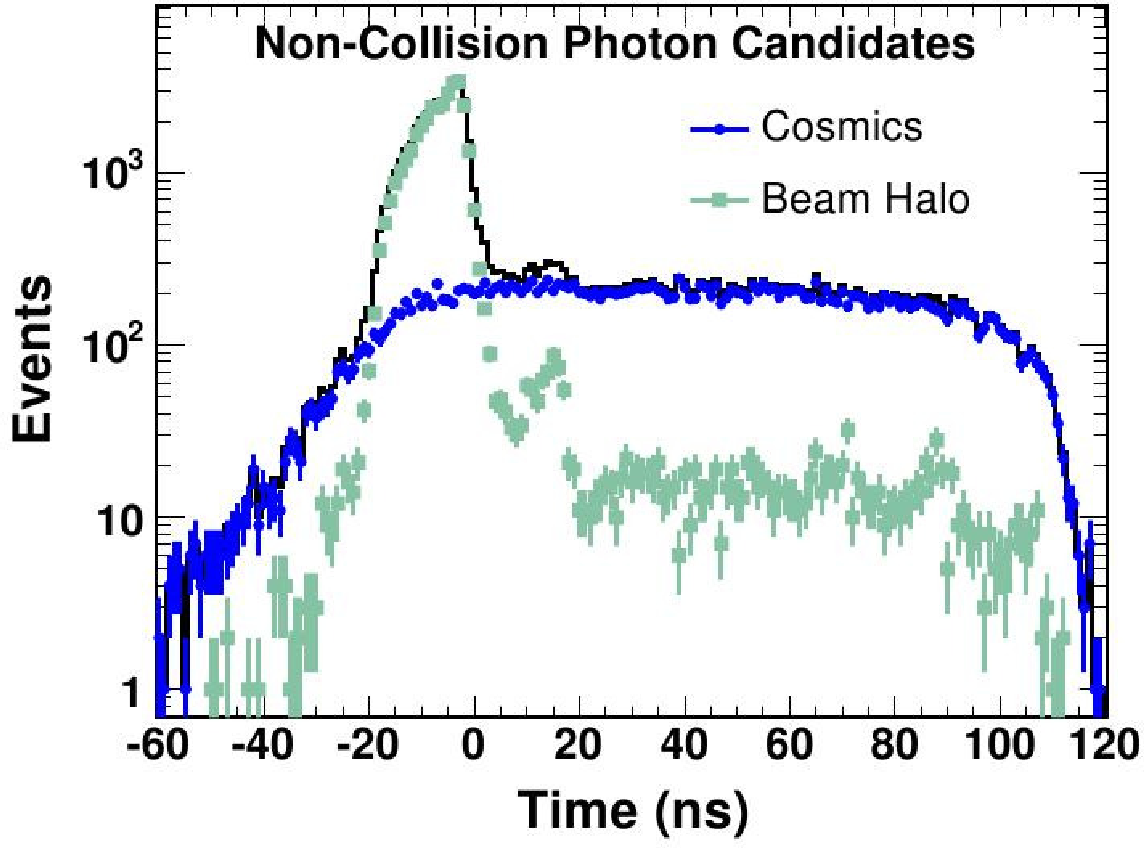
\includegraphics[scale=0.5]{./CosmicBeamHalo_EMtiming.pdf}
 % CosmicBeamHalo_EMtiming.pdf: 612x792 pixel, 72dpi, 21.59x27.94 cm, bb=0 0 612 792
 \caption[EM timing distribution of photon candidates.]{EM timing distribution of cosmic ray and beam halo photon candidates. Photon candidates from the hard scattering process arrive at the EM calorimeter around $t=0$~ns. A beam halo photon candidate reaches the EM calorimeter slightly earlier as its path is shorter than that of a photon candidate from a collision. The beam halo photon candidates from the satellite bunches can also be seen in intervals of 18~ns. Cosmic ray photon candidates are created at a constant rate that is independent of the hard scattering rate. This is indicated by the constant EM timing measurements of cosmic ray photon candidates.}
 \label{fig:CosmicBeamHaloEMtiming}
\end{figure}

\subsubsection{Rejection Power of the Beam Halo Selection Requirements}
The fraction of beam halo events identified and removed by beam halo selection requirements, also known as the \newterm{rejection power} of the beam halo selection requirements, is calculated by isolating a sample rich in beam halo events and determining the fraction of events that can be identified by these selection requirements. For this, a sample of events from data is selected following the criteria in Table~\ref{tab:HaloRejecCalcSelection}.

\begin{table}[hptm]
\caption{Summary of the event selection used to measure the rejection power of the beam halo selection requirements.}
\label{tab:HaloRejecCalcSelection}
\centering
 \begin{tabular}{cc}
\hline
\BUbf{Selection Variable} & \BUbf{Requirement}\\
\hline
Goodrun & Pass\\
\multirow{2}{*}{Trigger} & Pass any one of the triggers\\
& \firstphotrig, \secondphotrig, \thirdphotrig \\
Primary Vertices & $=0$ (No vertices)\\[2ex]
\sc{Photon Selection} & $E_{T}^{\gamma} > 30$~\etUnits, $|\eta_{detector}^{\gamma}|<1.1$\\
& Pass tight photon\\
& selection requirements (see Table~\ref{tab:tightAndLoosePhotonCuts})\\[2ex]
EM timing & $|\Delta t^{\gamma}|<4.8$~ns\\
Tracks (Phoenix) & No phoenix tracks\\
Muon stubs & 0 (No muon stubs)\\[2ex]
\sc{Jet Selection} & No requirement on number of jets\\
Jet--\met separation & N/A\\
\hline
 \end{tabular}
\end{table}

\begin{figure}[htbm]
 \centering
 \subfigure[]{
 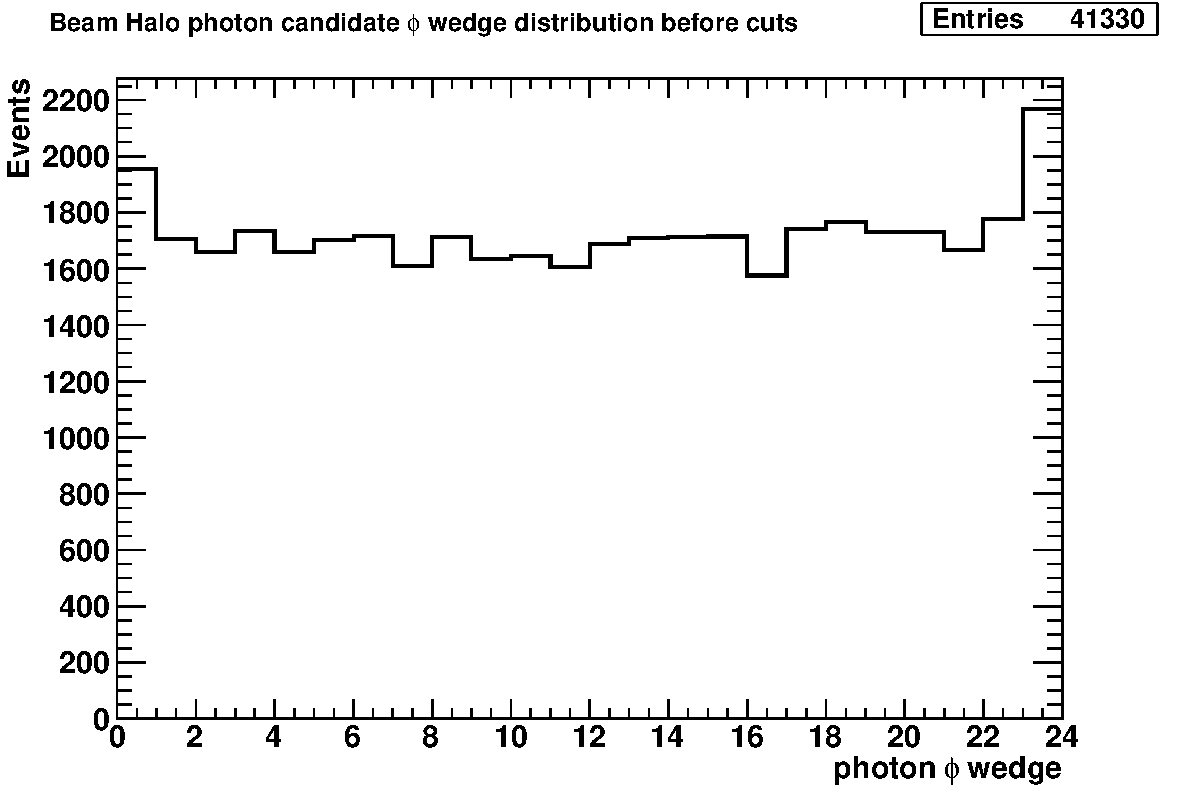
\includegraphics[scale=0.35,keepaspectratio=true]{./haloRejPow_b4cuts.pdf}
 % haloRejPow_b4cuts.pdf: 567x384 pixel, 72dpi, 20.00x13.55 cm, bb=0 0 567 384
}
 \subfigure[]{
 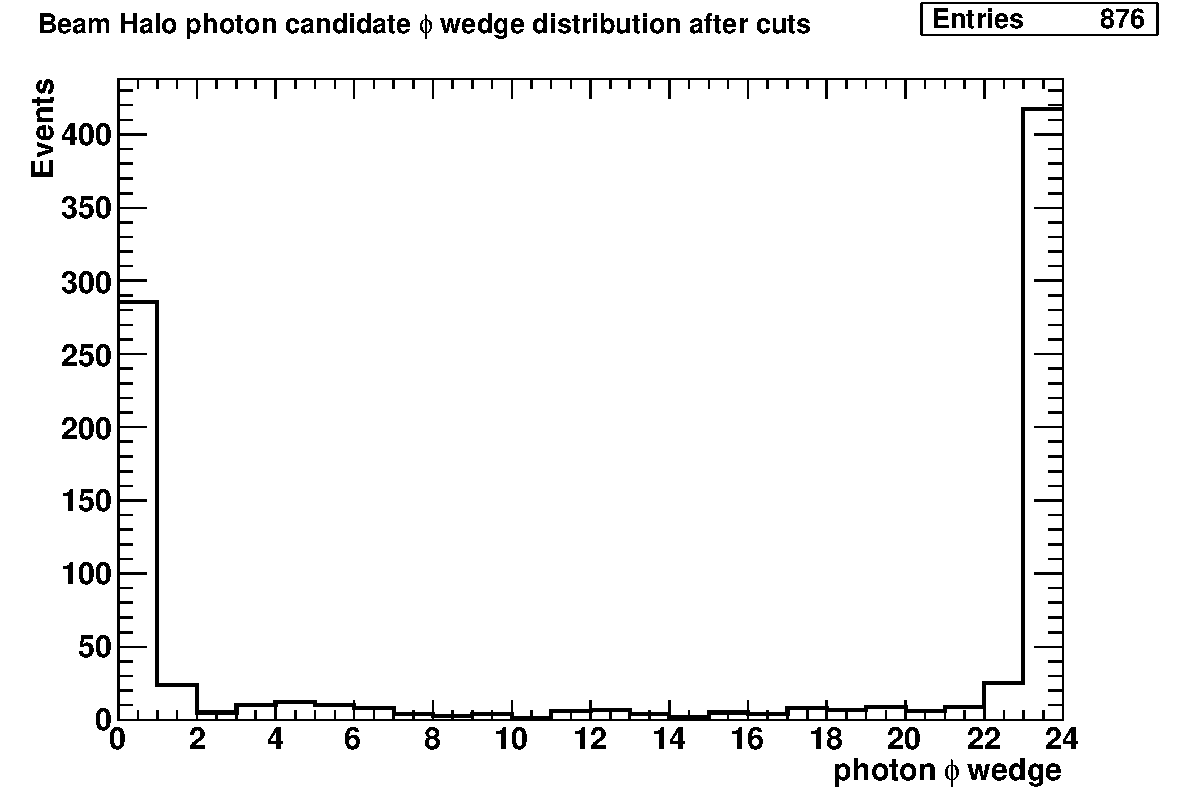
\includegraphics[scale=0.35,keepaspectratio=true]{./haloRejPow_a4cuts.pdf}
}
\caption{$\phi$ wedge distribution of the beam halo photon candidates before and after the beam halo selection requirements are applied.}
 \label{fig:BHrej_PhoPhiWedge}
\end{figure}

The selected events with no primary vertex are mostly beam halo and cosmic events. Beam halo selection requirements are applied to this sample of events to determine the event distribution in $\phi$ wedges of the leading photon (see Fig.~\ref{fig:BHrej_PhoPhiWedge}). Then, events in $\phi$ wedges 0 and 23 are counted and the flat component (misidentified cosmic events), estimated from the $\phi$ wedges 1 through 22, is subtracted. The beam halo rejection power can be calculated using
\begin{eqnarray}
 \mathrm{Beam~Halo~Rejection~Power}~(R^{Halo})&=& \frac{N_{0}^{a} - {2\bar{N}_{1}^{a} }}{N_{0}^{b} - {2\bar{N}_{1}^{b} }}\\
 &=& \frac{{286 + 417- 2\times \frac{173}{22}}}{1954 + 2168 - 2 \times \frac{37208}{22}} \nonumber\\
 &=& 92.9\%
\label{eqa:HaloRejectionPower}
\end{eqnarray}
where $N_{0}^{a}$ ($N_{0}^{b}$) is the aggregate number of events in wedges 0 and 23 after (before) the selection requirements are applied and $\bar{N}_{1}^{a}$ ($\bar{N}_{1}^{b}$) is the average number of events in wedges 1 through 22 after (before) the selection requirements are applied. This is evaluated using an inclusive \phoonejet data sample.

The percentage of beam halo events that are not removed is $1-R^{Halo} = 7.1\%$. An estimate of the remaining beam halo photons in the data sample can be estimated according to the same procedure by using the $\phi$ wedge distribution of the beam halo photon candidates identified using beam halo selection requirements, as described by
\begin{eqnarray}
 \mathrm{Expected~Beam~Halo~Events}~(N^{Halo})&=& (N_{0} - 2\bar{N_{1}}) (1-R^{Halo})
\label{eqa:HaloEstimate}
\end{eqnarray}
where $N_{0}$ is the number of events in $\phi$ wedges 0 and 23 and $\bar{N_{1}}$ is the average number of events in $\phi$ wedges 1 through 22.

\subsubsection{Misidentification Rate of the Beam Halo Selection Requirements}
As with any set of selection requirements, the beam halo selection requirements will occasionally misidentify real photon candidates from the primary collision as beam halo photons. This misidentification rate is measured using electrons, as electrons are produced often in the collisions and are more readily identifiable by their associated track. First, a sample of events with an electron + $\geq$1~jet is identified using photon-like electron selection requirements (see Table~\ref{tab:pecuts}). The electron + jet selection criteria is identical to that of the photon + jets selection. The electron should have \etg{30.0} and \etalessthan{1.1} and the jet should have \etg{15} and \etalessthan{3.0}. Finally, the beam halo selection requirements are applied to the electron in the events and the number of events that pass the selection requirements are counted. The following equation calculates the misidentification rate of the beam halo selection requirements:
\begin{eqnarray}
\mathrm{Beam~Halo~Misidentification~Rate}~(M^{Halo}) &=& \frac{N^{e+jets}_{after}}{N^{e+jets}_{before}}\\
 &=& 1.2\%
\label{eqa:HaloMisIdRate}
\end{eqnarray}
\noindent where $N^{e+jets}_{before}$ is the total number of identified electron + jets events and $N^{e+jets}_{after}$ is the number of electron + jets events identified as beam halo candidates (by passing the beam halo selection requirements).

The choice of beam halo selection requirements is a compromise between rejection power and misidentification rate. This low misidentification rate is a good choice as almost 95\% of beam halo events are rejected at a loss of only about 1\% of real photon events. The misidentification rate increases slightly with extra jets and interactions. The effect is less than a percent. Since the overall background expectation is very small, the rejection power is not reevaluated for these subsamples.

\subsubsection{Beam Halo Photon Template}
In order to model the distribution (shape) of the remaining beam halo events in the signal sample, a template is made and properly scaled to the expected number of beam halo events.

A beam halo template is made by selecting data events with criteria listed in Table~\ref{tab:HaloTempSelection}. This template is scaled to the expected number of beam halo events in data.

\begin{table}[htmb]
\caption{Summary of the event selection used to model the beam halo background.}
\label{tab:HaloTempSelection}
\centering
 \begin{tabular}{cc}
\hline
\BUbf{Selection Variable} & \BUbf{Requirement}\\
\hline
Goodrun & Pass\\[1ex]
\multirow{2}{*}{Trigger} & Pass any one of the triggers\\
& \firstphotrig, \secondphotrig, \thirdphotrig \\[1ex]
Primary Vertices & $=0$ (No vertices)\\[2ex]
\sc{Photon Selection} & $E_{T}^{\gamma} > 30$~\etUnits, $|\eta_{detector}^{\gamma}|<1.1$\\
& Pass tight photon\\
& selection requirements (see Table~\ref{tab:tightAndLoosePhotonCuts})\\[2ex]
EM timing & $|\Delta t^{\gamma}|<4.8$~ns\\
Tracks (Phoenix) & No phoenix tracks\\
Muon stubs & 0 (No muon stubs)\\[2ex]
Beam halo selection requirements & Pass\\
$\phi$-wedge & 0 or 23 only\\[2ex]
\sc{Jet Selection} & $\geq1$ jet with $E_{T}^{jet} > 15$~\etUnits, $|\eta_{detector}^{jet}|< 3.0$\\
Jet--\met separation & $\Delta \phi(\met - \mathrm{jet})>0.4$\\
\hline
 \end{tabular}
\end{table}

%%%%%%%%%%%%%%%%%%%%%%%%%%%%%%%%%%%%%%%%%%%%%%%%%%%%%%%%%%%%%%%%%%%%%
%     COSMIC PHOTON BACKGROUND
%%%%%%%%%%%%%%%%%%%%%%%%%%%%%%%%%%%%%%%%%%%%%%%%%%%%%%%%%%%%%%%%%%%%%

\subsubsection{Cosmic Photons}\label{sec:cosmicjets}
Occasionally, a cosmic ray (extraterrestrial high energy muon passing through the earth) interacts with the calorimeter and undergoes bremsstrahlung to create a fake photon candidate. This is called a \newterm{cosmic photon}. These muons are also likely to cross calorimeter towers separated in $\eta$ and $\Phi$ from the photon candidate. Hence, there is a chance that they will deposit enough energy in those towers to produce a reconstructible soft jet or even another photon.

The cosmic photon background is a constant-rate background that is independent of the time of the collision as seen in Fig.~\ref{fig:CosmicBeamHaloEMtiming}. These events can give rise to a large energy imbalance in the event, and hence tend to occupy the large missing energy region. By requiring the arrival time of the photon candidate from the primary collision to be \intimewindow, most of the cosmic photon events are removed. Such events are further removed by identifying muon stubs around a 30\degree cone of the photon candidate \cite{cdfnote:7960, cdfnote:8409}. The first 400~\pbi of Run II data is not used because it does not have EM timing information to reject this background effectively.

The number of cosmic photon events in the data sample is estimated using the EM timing distribution of the photon candidates using the equation
\begin{equation}
\mathrm{Cosmic~Photon~Estimate}~(N^{Cosmic}) = \frac{N_{30-90}^{cosmic}}{90~\mathrm{ns} - 30~\mathrm{ns}} \times (4.8~\mathrm{ns}\times2)
\label{eqn:cosmicEstimate}
\end{equation}
where $N_{30-90}^{cosmic}$ is the number of photon + jet events with an EM timing of the photon between 30--90~ns, selected using the criteria summarized in Table~\ref{tab:CosmicPhoSelection}.

Equation~\ref{eqn:cosmicEstimate} counts the number of cosmic photon candidate events in the time window between \cosmictimewindow and then extrapolates it to the \intimewindow time window, from which events in data are selected.

\subsubsection{Cosmic Photon Template}
A template for the cosmic photon background is made by selecting data events that satisfy the requirements in Table~\ref{tab:CosmicPhoSelection} and normalizing to the expected number of events ($N^{Cosmic}$).

\begin{table}[htmb]
\caption{Summary of the event selection used to estimate and model the cosmic photon background.}
\label{tab:CosmicPhoSelection}
\centering
 \begin{tabular}{cc}
\hline
\BUbf{Selection Variable} & \BUbf{Requirement}\\
\hline
Goodrun & Pass\\[2ex]
\multirow{2}{*}{Trigger} & Pass any one of the triggers\\
& \firstphotrig, \secondphotrig, \thirdphotrig \\[2ex]
Primary Vertices & $=0$ (No vertices)\\[2ex]
\sc{Photon Selection} & $E_{T}^{\gamma} > 30$~\etUnits, $|\eta_{detector}^{\gamma}|<1.1$\\
& Pass tight photon\\
& selection requirements (see Table~\ref{tab:tightAndLoosePhotonCuts})\\[2ex]
EM timing & $+30~\mathrm{ns} <\Delta t^{\gamma} < +90$~ns\\
Tracks (Phoenix) & No phoenix tracks\\
Muon stubs & 0 (No muon stubs)\\
Beam halo selection requirements & Fail\\[2ex]
\sc{Jet Selection} & $\geq$1 jet with $E_{T}^{jet} > 15$~\etUnits, $|\eta_{detector}^{jet}|< 3.0$\\
Jet--\met separation & $\Delta \phi(\met - \mathrm{jet})>0.4$\\
\hline
 \end{tabular}
\end{table}

\section{Method B}\label{sec:AltBgPrediction}
In an attempt to overcome the limitations of using a leading-order Monte Carlo generator to model jet properties in $\gamma$ + jets events, a novel method is implemented in which the QCD multijet events from the sideband data are used as a substitute for the \pythiaText SM $\gamma$ events. Although the QCD multijet events originate from a different physical process than prompt $\gamma$ + jets events, it is hypothesized that these events, which come from actual data, describe the properties of jets in $\gamma$ + jets events better than leading-order Monte Carlo. This should be readily apparent in distributions such as $H_T$ and the number of jets in the event.

Since the sideband data presumably do not contain actual prompt photons, and are only QCD background, one cannot expect the reconstructed ``QCD photons'' in those events to have the same \et distribution as the actual prompt photons from \pythiaText. The events in the QCD background template are therefore weighted in such a way that the weighted QCD template matches the sum of the \pythiaText SM $\gamma$ and QCD templates for the photon \et distribution. For an event in bin $i$ of the photon \et distribution, the associated weight is

\begin{equation}
w_i = \frac{N_i^{SM \gamma} + N_i^{QCD}}{N_i^{QCD}}\label{eqa:MtdBweight}
\end{equation}

\noindent where $N_i^{SM \gamma}$ and $N_i^{QCD}$ are the contents of each bin $i$ of the background templates determined using Method~A. Using Eq.~\ref{eqa:MtdBweight}, a unique weight can be assigned to every event in the QCD background sample based on the bin $i$ of the QCD photon \et. The effect of this reweighting on the sideband events is demonstrated in Fig.~\ref{fig:MtdB_Rewgt_Demo}. The actual weights and the fit is shown in Fig.~\ref{fig:MtdB_NominalWgts}.

\begin{figure}[p]
 \centering
\subfigure[]{
 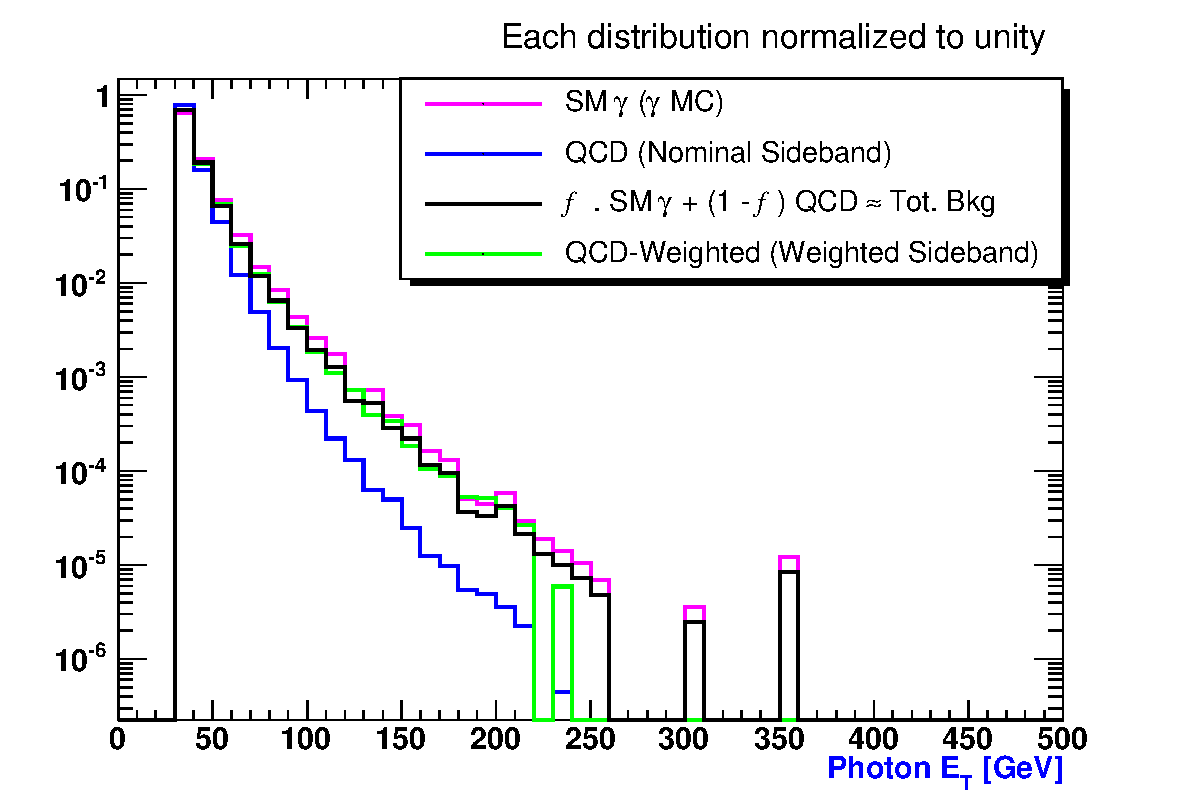
\includegraphics[scale=0.6,keepaspectratio=true]{./MtbB_RewgtDemo_PhoEt.pdf}
 % MtbB_RewgtDemo_PhoEt.pdf: 567x384 pixel, 72dpi, 20.00x13.55 cm, bb=0 0 567 384
}
\subfigure[]{
 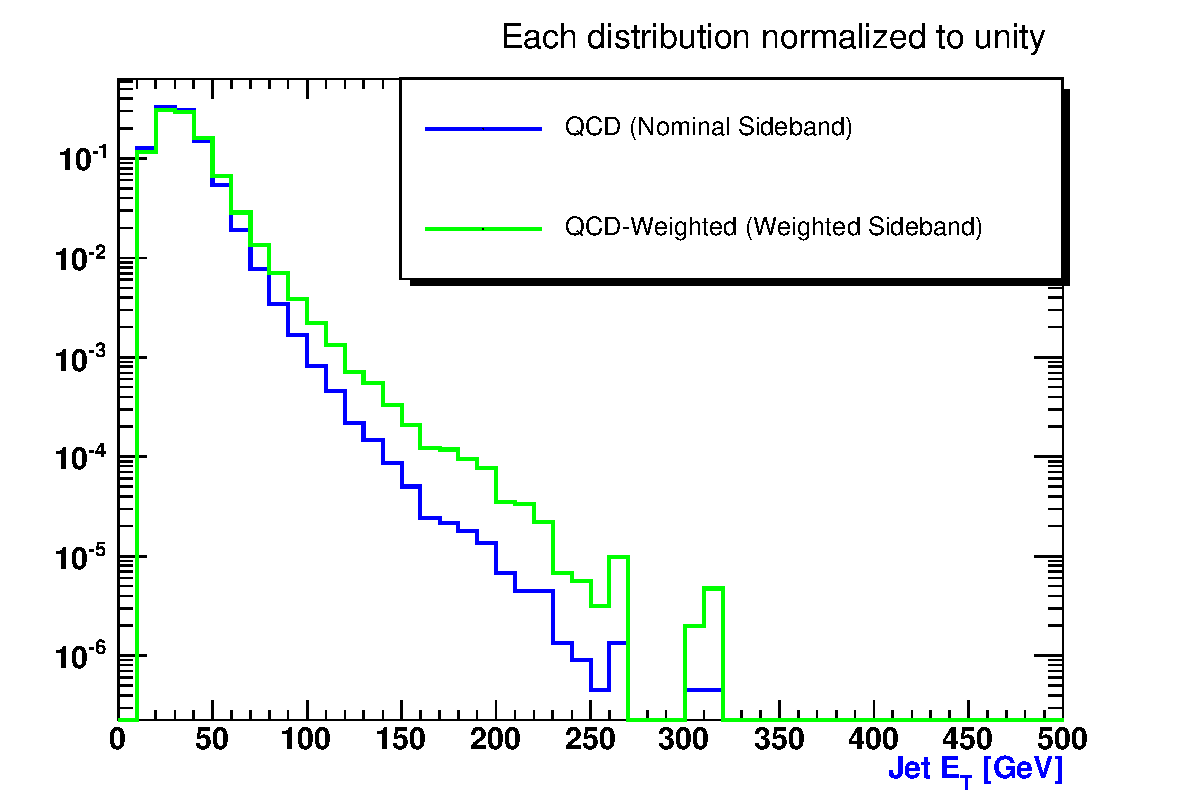
\includegraphics[scale=0.6,keepaspectratio=true]{./MtbB_RewgtDemo_JetEt.pdf}
 % MtbB_RewgtDemo_JetEt.pdf: 567x384 pixel, 72dpi, 20.00x13.55 cm, bb=0 0 567 384
}

 \caption{The effect of reweighting sideband events used in Method B. Every distribution shown is normalized to unit area for clarity. (a) The photon \et distributions of SM $\gamma$ (pink) and QCD (blue) are shown. The combination of the two distributions, according to the fake photon fraction, is shown in black. After the reweighting, the blue line becomes the green line. The green and black lines do not completely overlap due to the fact that the final weights are taken from a function fit to the binned data. (b) Sample plot showing how the photon \et weighting affects the leading jet in sideband events.}
\label{fig:MtdB_Rewgt_Demo}
\end{figure}

\begin{figure}[htb!]
 \centering
 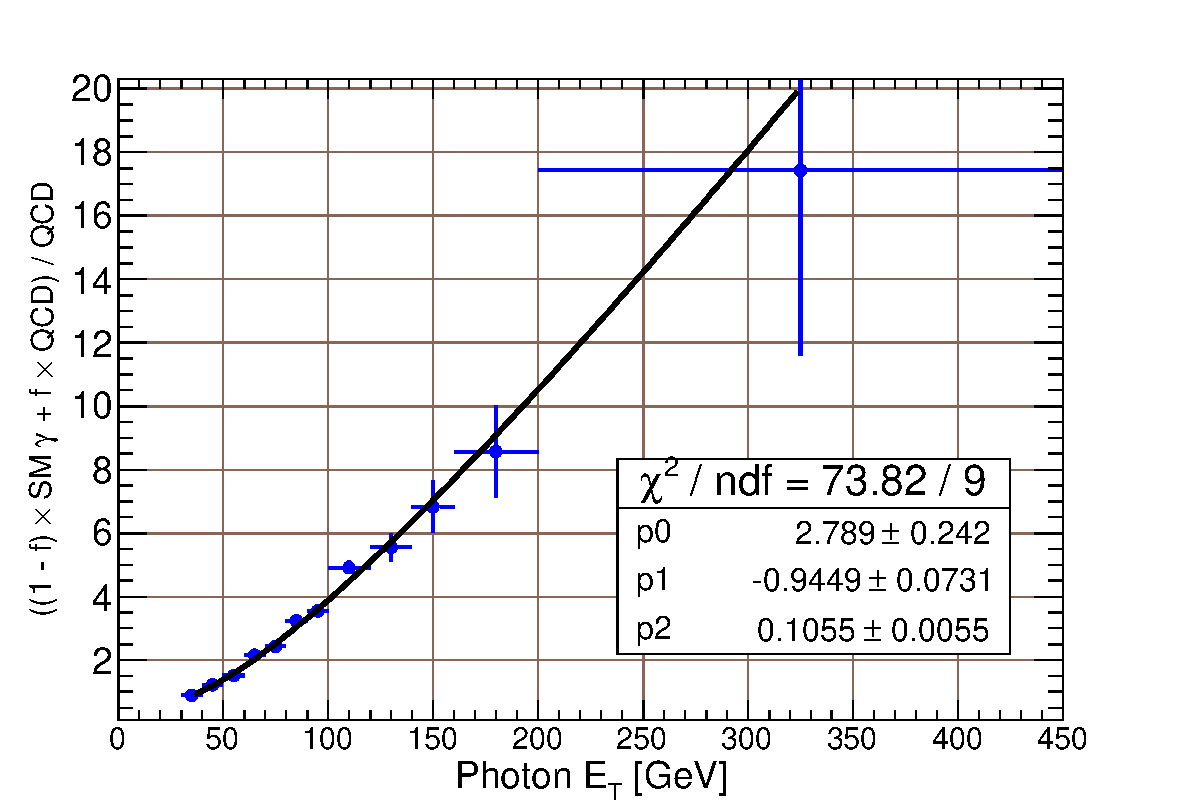
\includegraphics[scale=0.5,keepaspectratio=true]{./MtdB_Sideband_Weights.pdf}
 % MtdB_Sideband_Weights.pdf: 567x384 pixel, 72dpi, 20.00x13.55 cm, bb=0 0 567 384
 \caption{Distribution of weights used to reweight the sideband events in Method B. The functional form is $F(E_{T}^{\gamma},f)= p0+p1\times\sqrt{E_{T}^{\gamma}}+p2\times E_{T}^{\gamma}$.}
 \label{fig:MtdB_NominalWgts}
\end{figure}

By defining a weight in this manner for every QCD background event, the QCD background template can be weighted for every kinematic distribution. In all of the kinematic distributions, the weighted QCD template replaces the standard QCD template and the SM $\gamma$ template. In the case of photon \et, by definition, the weighted QCD background template will be identical to the sum of the SM $\gamma$ and QCD templates.

This weighting procedure is referred to as Method B. The weighted QCD template is normalized so that the total number of events, $N^\mathrm{Weighted-QCD}$, satisfies:
\begin{equation}
 N^\mathrm{Data} = N^\mathrm{Weighted-QCD}+\underbrace{N^\mathrm{Di-\gamma}}_{fixed}+\underbrace{N^\mathrm{EWK}}_{fixed}+\underbrace{N^\mathrm{Non-collision}}_{fixed}.
\label{eqa:MtdBnorm}
\end{equation}
As in Method A, the total number of background events is forced to be equal to the total number of data events in each data sample studied. An additional systematic uncertainty has been calculated for the weighting procedure, and it is included in the Method B distributions.
